% Options for packages loaded elsewhere
\PassOptionsToPackage{unicode}{hyperref}
\PassOptionsToPackage{hyphens}{url}
\PassOptionsToPackage{dvipsnames,svgnames,x11names}{xcolor}
%
\documentclass[
  10pt,
  dvipsnames,enabledeprecatedfontcommands]{scrartcl}
\usepackage{amsmath,amssymb}
\usepackage{lmodern}
\usepackage{iftex}
\ifPDFTeX
  \usepackage[T1]{fontenc}
  \usepackage[utf8]{inputenc}
  \usepackage{textcomp} % provide euro and other symbols
\else % if luatex or xetex
  \usepackage{unicode-math}
  \defaultfontfeatures{Scale=MatchLowercase}
  \defaultfontfeatures[\rmfamily]{Ligatures=TeX,Scale=1}
\fi
% Use upquote if available, for straight quotes in verbatim environments
\IfFileExists{upquote.sty}{\usepackage{upquote}}{}
\IfFileExists{microtype.sty}{% use microtype if available
  \usepackage[]{microtype}
  \UseMicrotypeSet[protrusion]{basicmath} % disable protrusion for tt fonts
}{}
\usepackage{xcolor}
\usepackage{graphicx}
\makeatletter
\def\maxwidth{\ifdim\Gin@nat@width>\linewidth\linewidth\else\Gin@nat@width\fi}
\def\maxheight{\ifdim\Gin@nat@height>\textheight\textheight\else\Gin@nat@height\fi}
\makeatother
% Scale images if necessary, so that they will not overflow the page
% margins by default, and it is still possible to overwrite the defaults
% using explicit options in \includegraphics[width, height, ...]{}
\setkeys{Gin}{width=\maxwidth,height=\maxheight,keepaspectratio}
% Set default figure placement to htbp
\makeatletter
\def\fps@figure{htbp}
\makeatother
\setlength{\emergencystretch}{3em} % prevent overfull lines
\providecommand{\tightlist}{%
  \setlength{\itemsep}{0pt}\setlength{\parskip}{0pt}}
\setcounter{secnumdepth}{5}
\newlength{\cslhangindent}
\setlength{\cslhangindent}{1.5em}
\newlength{\csllabelwidth}
\setlength{\csllabelwidth}{3em}
\newlength{\cslentryspacingunit} % times entry-spacing
\setlength{\cslentryspacingunit}{\parskip}
\newenvironment{CSLReferences}[2] % #1 hanging-ident, #2 entry spacing
 {% don't indent paragraphs
  \setlength{\parindent}{0pt}
  % turn on hanging indent if param 1 is 1
  \ifodd #1
  \let\oldpar\par
  \def\par{\hangindent=\cslhangindent\oldpar}
  \fi
  % set entry spacing
  \setlength{\parskip}{#2\cslentryspacingunit}
 }%
 {}
\usepackage{calc}
\newcommand{\CSLBlock}[1]{#1\hfill\break}
\newcommand{\CSLLeftMargin}[1]{\parbox[t]{\csllabelwidth}{#1}}
\newcommand{\CSLRightInline}[1]{\parbox[t]{\linewidth - \csllabelwidth}{#1}\break}
\newcommand{\CSLIndent}[1]{\hspace{\cslhangindent}#1}
%\documentclass{article}

% %packages
 \usepackage{booktabs}
\usepackage{subcaption}
\usepackage{multirow}
\usepackage{colortbl}
\usepackage{graphicx}
\usepackage{longtable}
\usepackage{ragged2e}
\usepackage{etex}
%\usepackage{yfonts}
\usepackage{marvosym}
\usepackage[notextcomp]{kpfonts}
\usepackage{nicefrac}
\newcommand*{\QED}{\hfill \footnotesize {\sc Q.e.d.}}
\usepackage{floatrow}
%\usepackage[titletoc]{appendix}
%\renewcommand\thesubsection{\Alph{subsection}}

\usepackage[textsize=footnotesize]{todonotes}
\newcommand{\ali}[1]{\todo[color=gray!40]{#1}}
\newcommand{\mar}[1]{\todo[color=blue!40]{#1}}
\newcommand{\raf}[1]{\todo[color=olive!40]{#1}}
%\linespread{1.5}
\newcommand{\indep}{\!\perp \!\!\! \perp\!}


\setlength{\parindent}{10pt}
\setlength{\parskip}{1pt}


%language
\usepackage{times}
\usepackage{t1enc}
%\usepackage[utf8x]{inputenc}
%\usepackage[polish]{babel}
%\usepackage{polski}




%AMS
\usepackage{amsfonts}
\usepackage{amssymb}
\usepackage{amsthm}
\usepackage{amsmath}
\usepackage{mathtools}

\usepackage{geometry}
 \geometry{a4paper,left=35mm,top=20mm,}


%environments
\newtheorem{fact}{Fact}



%abbreviations
\newcommand{\ra}{\rangle}
\newcommand{\la}{\langle}
\newcommand{\n}{\neg}
\newcommand{\et}{\wedge}
\newcommand{\jt}{\rightarrow}
\newcommand{\ko}[1]{\forall  #1\,}
\newcommand{\ro}{\leftrightarrow}
\newcommand{\exi}[1]{\exists\, {_{#1}}}
\newcommand{\pr}[1]{\mathsf{P}(#1)}
\newcommand{\cost}{\mathsf{cost}}
\newcommand{\benefit}{\mathsf{benefit}}
\newcommand{\ut}{\mathsf{ut}}

\newcommand{\odds}{\mathsf{Odds}}
\newcommand{\ind}{\mathsf{Ind}}
\newcommand{\nf}[2]{\nicefrac{#1\,}{#2}}
\newcommand{\R}[1]{\texttt{#1}}
\newcommand{\prr}[1]{\mbox{$\mathtt{P}_{prior}(#1)$}}
\newcommand{\prp}[1]{\mbox{$\mathtt{P}_{posterior}(#1)$}}

\newcommand{\s}[1]{\mbox{$\mathsf{#1}$}}


\newtheorem{q}{\color{blue}Question}
\newtheorem{lemma}{Lemma}
\newtheorem{theorem}{Theorem}



%technical intermezzo
%---------------------

\newcommand{\intermezzoa}{
	\begin{minipage}[c]{13cm}
	\begin{center}\rule{10cm}{0.4pt}



	\tiny{\sc Optional Content Starts}
	
	\vspace{-1mm}
	
	\rule{10cm}{0.4pt}\end{center}
	\end{minipage}\nopagebreak 
	}


\newcommand{\intermezzob}{\nopagebreak 
	\begin{minipage}[c]{13cm}
	\begin{center}\rule{10cm}{0.4pt}

	\tiny{\sc Optional Content Ends}
	
	\vspace{-1mm}
	
	\rule{10cm}{0.4pt}\end{center}
	\end{minipage}
	}
%--------------------






















\newtheorem*{reply*}{Reply}
\usepackage{enumitem}
\newcommand{\question}[1]{\begin{enumerate}[resume,leftmargin=0cm,labelsep=0cm,align=left]
\item #1
\end{enumerate}}

\usepackage{float}

% \setbeamertemplate{blocks}[rounded][shadow=true]
% \setbeamertemplate{itemize items}[ball]
% \AtBeginPart{}
% \AtBeginSection{}
% \AtBeginSubsection{}
% \AtBeginSubsubsection{}
% \setlength{\emergencystretch}{0em}
% \setlength{\parskip}{0pt}






\usepackage[authoryear]{natbib}

%\bibliographystyle{apalike}



\usepackage{tikz}
\usetikzlibrary{positioning,shapes,arrows}

\ifLuaTeX
  \usepackage{selnolig}  % disable illegal ligatures
\fi
\IfFileExists{bookmark.sty}{\usepackage{bookmark}}{\usepackage{hyperref}}
\IfFileExists{xurl.sty}{\usepackage{xurl}}{} % add URL line breaks if available
\urlstyle{same} % disable monospaced font for URLs
\hypersetup{
  pdftitle={Weight Chapter Outline},
  colorlinks=true,
  linkcolor={Maroon},
  filecolor={Maroon},
  citecolor={Blue},
  urlcolor={blue},
  pdfcreator={LaTeX via pandoc}}

\title{Weight Chapter Outline}
\author{}
\date{\vspace{-2.5em}9/1/2022}

\begin{document}
\maketitle

{
\hypersetup{linkcolor=}
\setcounter{tocdepth}{2}
\tableofcontents
}
\hypertarget{introduction}{%
\section{Introduction}\label{introduction}}

A defendant in a criminal case may face multiple items of incriminating
evidence, and their overall strength can sometimes be assessed using
probabilities. For example, suppose hair found at the crime scene
matches the defendant hair (call this evidence, \textsf{hair}). In
addition, the defendant owns a dog whose fur matches the dog fur found
in a carpet wrapped around one of the bodies (call this evidence,
\textsf{dog}).\footnote{The hair evidence and the dog fur evidence are
  stylized after two items of evidence in the notorious 1981 Wayne
  Williams case.}
\todo{CITE: H A Deadman, Fiber Evidence and the Wayne Williams Trial (Part I), FBI Law Enforcement Bulletin Volume: 53 Issue: 3 Dated: (March 1984) Pages: 12-20 and H A Deadman, Fiber Evidence and the Wayne Williams Trial (Conclusion), bFBI Law Enforcement Bulletin Volume:: 53 Issue: 5 Dated: (May 1984) Pages: 10-19.}
What are the fact-finders to make of this evidence?

To evaluate the strength of the evidence, an expert provides random
match probabilities for each item of match evidence. The expert
testifies that the probability of a random person's hair matching the
reference sample is about 0.0253, and the probability of a random dog's
hair matching the reference sample happens to be about the same,
0.0256.\footnote{Probabilities have been slightly but not
  unrealistically modified to be closer to each other in order to make a
  conceptual point. The original probabilities were 1/100 for the dog
  fur, and 29/1148 for Wayne Williams' hair. We modified the actual
  reported probabilities slightly to emphasize the point that we will
  elaborate further on: the same first-order probabilities, even when
  they sound precise, may be affected by second-order uncertainty to
  different extents.} Suppose these probabilities are independent of
each other conditional on the source hypothesis, namely that the
defendant (or the defendant's dog) is the source of the hair (or dog
fur) found at the scene (call this hypothesis, \(\mathsf{source}\))
Then, to evaluate the total impact of the evidence on the source
hypothesis, you calculate: \begin{align*}
\pr{\s{dog}\wedge \s{hair} \vert \neg \s{source}} & = \pr{\s{dog} \vert \neg \s{source}} \times \pr{\s{hair} \vert \neg \s{source}} \\
& =  0.0252613 \times  0.025641 = \ensuremath{6.4772626\times 10^{-4}}
\end{align*} This seems like a low number. To get a better grip on how
this should be interpreted, the expert shows you how the posterior
probability of the source hypothesis (based on the two two items of
match evidence) depends on the prior probabilities (Figure
\ref{fig:impactOfPoint}). The posterior of .99 is reached as soon as the
prior is higher than 0.061.\footnote{These calculations assume that the
  probability of a match if the suspect (or the suspect's dog) is the
  source is one.} While perhaps not sufficient for believing outright
the source hypothesis, the evidence is quite strong: a minor additional
piece of evidence could tip the scale against the defendant.

\begin{figure}[H]

\begin{center}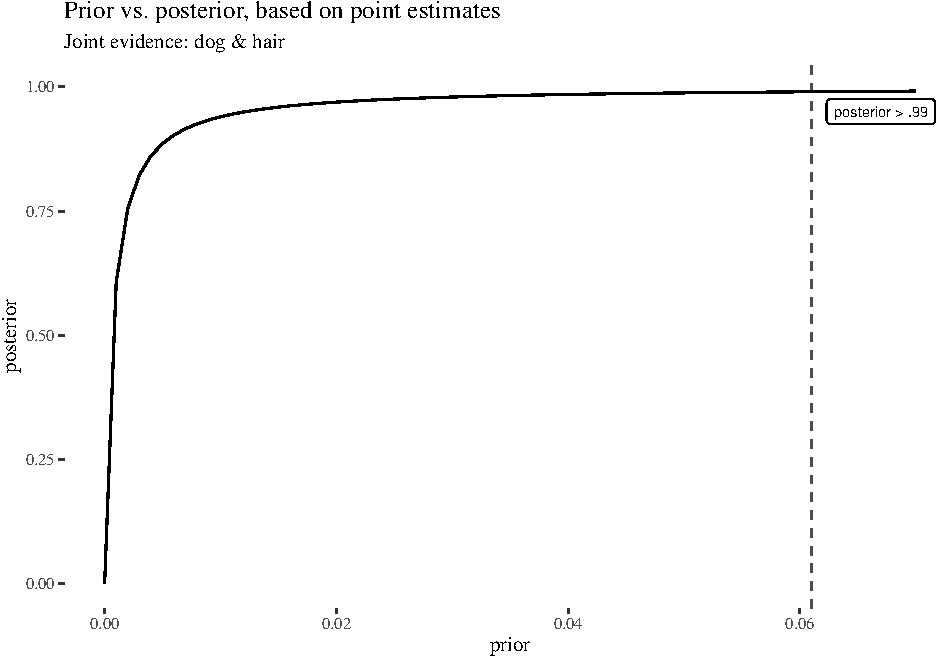
\includegraphics[width=0.8\linewidth]{chapter-outline_files/figure-latex/impactOfPoint4-1} \end{center}
\caption{Impact of dog fur and human hair evidence on the prior, point estimates.}
\label{fig:impactOfPoint}
\end{figure}

Unfortunately, such probabilistic assessment of the two items of match
evidence left out something crucial. You reflect on what you have been
told and ask the expert: how can you know these random match
probabilities with precision? Shouldn't we also be mindful of the
uncertainty about these numbers? The expert agrees, and tells you that
in fact the random match probability for the hair evidence is based on
29 matches found in a database of size 1148, while the random match
probability for the dog evidence is based on finding two matches in a
reference database of size 78.

The expert's answer makes apparent that that precise random match
probabilities do not tell the whole story. What to do, then? You ask the
expert for guidance: what are reasonable ranges of the random match
probabilities? What are the worst-case and best-case scenarios? The
expert responds with 99\% credible intervals---specifically, starting
with uniform priors, the ranges of the random match probabilities are
(.015,.037) for hair evidence and (.002, .103) for fur
evidence.\footnote{Roughly, the 99\% credible interval is the narrowest
  interval to which the expert thinks the true parameter belongs with
  probability .99. For a discussion of what credible intervals are; how
  they differ from confidence intervals; and why confidence intervals
  should not be used, see the discussion in Chapter XXX.}

With good intentions, you redo your calculations using the upper bounds
of the two intervals. Using the upper bounds would result in random
match probabilities that are most favorable to the defendant. That is,
\(\mathsf{P}_{def}(\s{dog}\wedge \s{hair} \vert \neg \s{source}) = .037 * .103 =.003811\).
This number is around 5.88 times greater than the original estimate
\ensuremath{6.4772626\times 10^{-4}}! Now the prior probability of the
source hypothesis needs to be higher than 0.274 for the posterior
probability to be above .99 (Figure \ref{fig:impactOfCharitable}). You
are no longer convinced that the two items of match evidence are strong
incriminating evidence.

\begin{figure}[H]

\begin{center}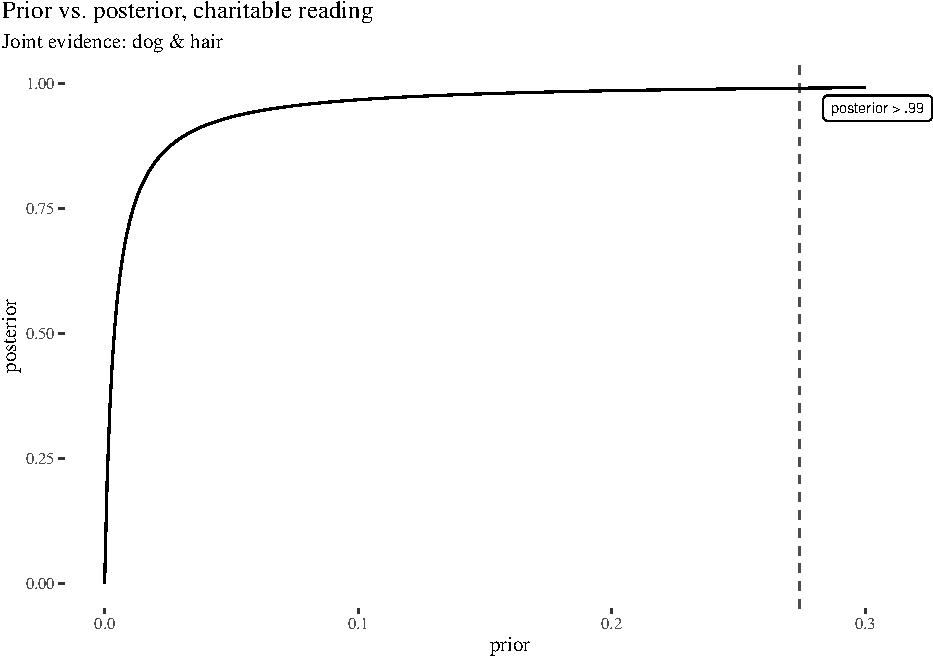
\includegraphics[width=0.8\linewidth]{chapter-outline_files/figure-latex/fig:charitableImpact7-1} \end{center}
\caption{Impact of dog fur and human hair evidence on the prior, charitable reading.}
\label{fig:impactOfCharitable}
\end{figure}

For one thing, it is clear that simply using precise random match
probabilities is too unfavorable toward the defendant. On the other
hand, you wonder whether your new assessment of the evidence is too
conservative and too favorable toward the defendant. The problem, then,
is to avoid underestimating and overestimating the value of the
evidence.

In your calculations, you made an important blunder. Just because the
worst-case probability for one event is \(x\) and the worst-case
probability for another independent event is \(y\), it does not follow
that the worst-case probability for their conjunction is \(xy\), if the
margin of error is kept fixed. The intuitive reason is simple: just
because the probability of an extreme (or larger absolute) value \(x\)
for one variable is .01, and so it is for the value \(y\) of another
independent variable, it does not follow that the probability that those
two independent variables take values \(x\) and \(y\) simultaneously is
the same. This probability is actually much smaller.

In fact, if you knew what distributions the expert used (it should have
been beta distributions in this context), you could work your way back
and calculate the .99 highest posterior density interval for the
conjunction, which is \((0.000023, 0.002760)\). The proper charitable
reading would then require the prior to be above .215 for the posterior
to be above .99. Still not enough to convict, but at least now we worked
out the consequences of the aleatory uncertainties involved provided the
margin of error is fixed. Is this good enough?

Well, it seems the interval presentation instead of doing us good led us
into error --- the general phenomenon is that intervals do \textbf{not}
contain enough information to reliably reason about such things as
margins of error.\footnote{There is some ambiguity here: one might think
  that a 99\% margin of error is the 99\% confidence interval known from
  classical statistics. There are various reasons not to use these,
  already discussed in Chapter 3. Another sense, in which we mean it
  here, is the range to which the true value belongs with posterior
  probability of 99\% given the evidence. Normally we mean highest
  posterior density intervals, that is the narrowest intervals with this
  property.} Even if we are happy with the interval that we obtained, we
will not be able to correctly obtain a new interval once a new item of
evidence is included. That is, unless we proceed through the densities.

Another problem is that looking at intervals might be useful if the
underlying distributions are fairly symmetrical. But in our case, they
might not be. For instance, Figure \ref{fig:densities} illustrates are
the beta densities for dog fur and human hair, together with
sampling-approximated density for the joint evidence. Crucially, the
distribution is not symmetric, and so switching the margin of error
moves the right edge of the interval much faster towards lower values.
If you were only informed about the edges of the interval, you would be
oblivious to such phenomena and the fact that the most likely value does
\textbf{not} simply lie in the middle between the edges of the interval.
Just because the parameter lies in an interval with some posterior
probability, it does not mean that the ranges near the edges of the
interval are equally likely---it still might be the case that the bulk
of the density is closer to one of the edges, and therefore relying on
the edges only might lead us to either overestimate or underestimate the
risk at play.

\begin{figure}[H]

\begin{center}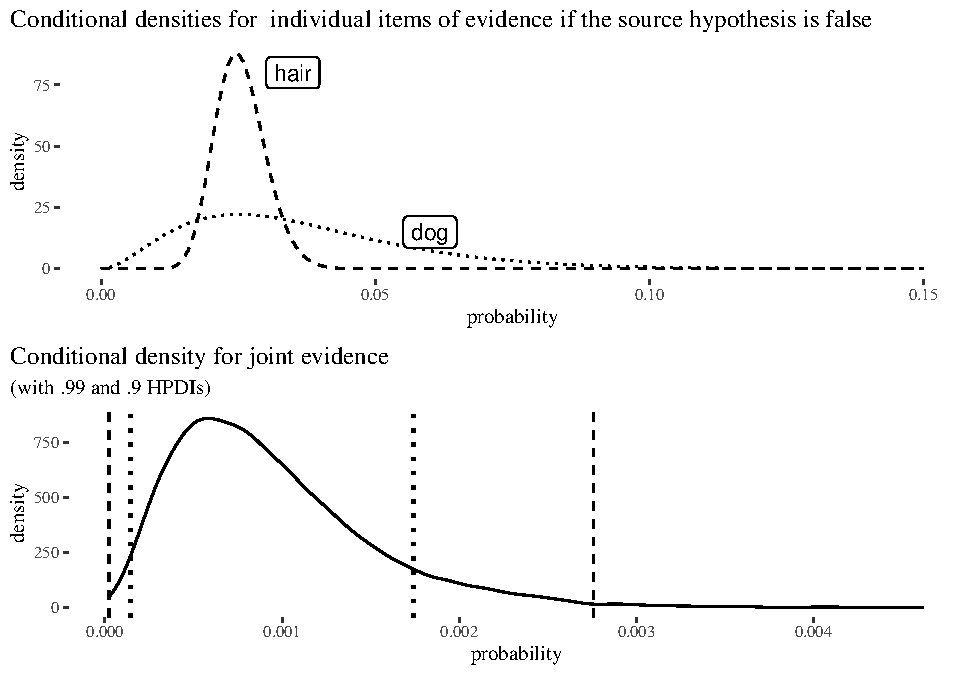
\includegraphics[width=0.8\linewidth]{chapter-outline_files/figure-latex/fig:densities-1} \end{center}
\caption{Beta densities for individual items of evidence and the resulting joint density with .99 and .9 highest posterior density intervals, assuming the sample sizes as discussed and independence, with uniform priors.}
\label{fig:densities}
\end{figure}

\todo{Revise this structure description once the chapter is done}

This is the gist of our chapter: whenever honest density estimates are
available (and they should be available for match evidence evaluation
methods whose reliability has been properly studied), it is those
densities that should be reported and used in further reasoning. This
avoids hiding actual aleatory uncertainties under the carpet, and allows
for more correct reasoning where interval-based representation might
either lead one astray or leave one oblivious to important probabilistic
considerations.

The rest of this chapter expands on this idea in a few dimensions.
First, it places it in the context of philosophical discussions
surrounding a proper probabilistic representation of uncertainty. The
main alternatives on the market are precise probabilism and imprecise
probabilism. We argue that both options are problematic and should be
superseded by the second-order representation whenever possible. Second,
having gained this perspective, we visit a recent discussion in the
forensic science literature, where a prominent proposal is that the
experts, even if they use densities, should integrate and present only
point estimates to the fact-finders. We disagree. Third, we explain how
the approach can be used in more complex situations in which multiple
items of evidence and multiple propositions interact---and the idea is
that such complexities can be handled by sampling from distributions and
approximating densities using multiple Bayesian Networks in the
calculations. Last but not least, we turn to the notion of weight of
evidence. Having distinguished quite a few notions in the vicinity, we
explain how the framework we propose allows for a more successful
explication and implementation of the notion of weight of evidence than
the ones currently available on the market.

\textbf{M's comment: On the structure of the chapter. So basically, the strcture of the chapter would be: (1) higher order approach in general, (2) illustration 1 (first application): DNA evidence debate Taroni, etc., (2) illustration 2 (second application): combing items of evidence, complex cases, etc. and (3)
illustration 3 (theory): modeling weight.}

\textbf{M's comment: We might concede that the higher order approach outlined in the introduction might not always be pratically useful, or its applicabiolity might be limited. Not sure. Need to discuss. Perhaps once the discussion about DNA evidence is in place, this will become more clear. One question might be: what kind of information do we need to get the higher order approach going? Regardless of its applicability---we can say, we want to leave this decision to practionares in the end---the higher order approach has important theorical significance because it allows to model notions such as weight.}

\hypertarget{three-probabilisms}{%
\section{Three probabilisms}\label{three-probabilisms}}

This section outlines three version of probabilism: precise, imprecise
and higher-order. Precise probabilism, as the name suggests, posits that
an agent' credal state is modeled by a single, precise probability
measure. Imprecise probabilism replaces precise probabilities by sets of
probability measures, while higher-order probabilism relies on
distributions over parameter values. There are good reasons to abandon
precise probabilism and endorse higher-order probabilism. Imprecise
probabilism is a step in the right direction, but as we will see, it
suffers from too many difficulties of its own.

\hypertarget{precise-probabilism}{%
\subsection{Precise Probabilism}\label{precise-probabilism}}

\textbf{Precise probabilism} (\textsf{PP}) holds that a rational agent's
uncertainty about a hypothesis \(H\) is to be represented as a single,
precise probability measure. This is an elegant and simple theory. But
representing our uncertainty about a proposition in terms of a single,
precise probability runs into a number of difficulties. Precise
probabilism fails to capture an important dimension of how our
uncertainty connects with the evidence we have or have not obtained.
Consider the following simple examples (we will be using examples with
coins for a bit, but the points are general and hold for all sampling
based frequency estimation methods, including those of random match
probability for various pieces of forensic evidence):

\begin{quote}
\textbf{No evidence v. fair coin}
You are about to toss a coin, but have no evidence 
whatsoever about its bias. You are completely ignorant.   Compare this to the situation  in which you know the coin is fair. 
\end{quote}

\noindent Sticking to \s{PP} you follow the principle of insufficient
evidence and assign probability .5 to the outcome being \emph{heads} in
both cases.

\begin{quote}
\textbf{Learning from ignorance}
You start  tossing the  coin with unknown bias, toss it ten times and observe \emph{heads} five times. You started with your bias estimate at .5, but you also end with your bias estimate at .5. Clearly, you have learned something, but whatever that is, it is not captured in the representation recommended by \s{PP}. Suppose you toss further, observing 50 \emph{heads} in 100 tosses. Again, your epistemic situation has changed, but it is hard to see how this shift could be represented on \s{PP}.
\end{quote}

\noindent Clearly, precise probabilism has difficulties modeling such
situations.\footnote{Examples of this sort date back to C. S. Peirce,
  who in his 1872 manuscript `The Fixation of Belief' (W3 295) comments:
  ``when we have drawn a thousand times, if about half {[}of the
  beans{]} have been white, we have great confidence in this result
  \ldots{} a confidence which would be entirely wanting if, instead of
  sampling the bag by 1000 drawings, we had done so by only two.'\,'
  Similar remarks can be found in Peirce's 1878
  \emph{Probability of Induction}. There, he also proposes to represent
  uncertainty by at least two numbers, the first depending on the
  inferred probability, and the second measuring the amount of knowledge
  obtained; as the latter, Peirce proposed to use some
  dispersion-related measure of error (but then suggested that an error
  of that estimate should also be estimated and so, so that ideally more
  numbers representing errors would be needed).} The examples suggest
that precise probabilism is not appropriately responsive to evidence. It
ends up assigning a probability of .5 to situations in which one's
evidence is quite different: when no evidence is available about the
coin's bias; when there is little evidence that the coin is fair (say,
after only 2 draws); when there is strong evidence that the coin is fair
(say, after 1000 draws).\footnote{Precise probabilism suffers from other
  difficulties. For example, it has problems with formulating a sensible
  method of probabilistic opinion aggregation Stewart \& Quintana
  (2018). A seemingly intuitive constraint is that if every member
  agrees that \(X\) and \(Y\) are probabilistically independent, the
  aggregated credence should respect this. But this is hard to achieve
  if we stick to \s{PP} (Dietrich \& List, 2016). For instance, a
  \emph{prima facie} obvious method of linear pooling does not respect
  this. Consider probabilistic measures \(p\) and \(q\) such that
  \(p(X) = p(Y) = p(X\vert Y) = 1/3\) and
  \(q(X) = q(Y) = q(X\vert Y) = 2/3\). On both measures, taken
  separately, \(X\) and \(Y\) are independent. Now take the average,
  \(r=p/2+q/2\). Then \(r(X\cap Y) = 5/18 \neq r(X)r(Y)=1/4\).}

\hypertarget{imprecise-probabilism}{%
\subsection{Imprecise Probabilism}\label{imprecise-probabilism}}

What if we give up the assumption that probability assignments should be
precise? \textbf{Imprecise probabilism} (\textsf{IP}) holds that an
agent's credal stance towards a hypothesis \(H\) is to be represented by
means of a \emph{set of probability measures}, typically called a
representor \(\mathbb{P}\), rather than a single measure \(\mathsf{P}\).
The representor should include all and only those probability measures
which are compatible (in a sense to be specified) with the evidence. For
instance, if an agent knows that the coin is fair, their credal state
would be captured by the singleton set \(\{\mathsf{P}\}\), where
\(\mathsf{P}\) is a probability measure which assigns \(.5\) to
\emph{heads}. If, on the other hand, the agent knows nothing about the
coin's bias, their credal state would rather be represented as the set
of all probabilistic measures, as none of them is excluded by the
available evidence. Note that the set of probability measures does not
represent admissible options that the agent could legitimately pick
from. Rather, the agent's credal state is essentially imprecise and
should be represented by means of the entire set of probability
measures.\footnote{For the development of imprecise probabilism, see
  (Fraassen, 2006; Gärdenfors \& Sahlin, 1982; Joyce, 2005; Kaplan,
  1968; Keynes, 1921; Levi, 1974; Sturgeon, 2008; Walley, 1991), (S.
  Bradley, 2019) is a good source of further references.}

Imprecise probabilism, at least \emph{prima facie}, offers a
straightforward picture of learning from evidence, that is a natural
extension of the classical Bayesian approach. When faced with new
evidence \(E\) between time \(t_0\) and \(t_1\), the representor set
should be updated point-wise, running the standard Bayesian updating on
each probability measure in the representor:\footnote{Imprecise
  probabilism shares some similarities with what we might call
  \textbf{interval probabilism} due to (Kyburg, 1961; Kyburg Jr \& Teng,
  2001). On interval probabilism, precise probabilities are replaced by
  intervals of probabilities. On imprecise probabilism, instead, precise
  probabilities are replaced by sets of probabilities. This makes
  imprecise probabilism more general, since the probabilities of a
  proposition in the representor set do not have to form a closed
  interval. Moreover, learning on Kyburg's approach is somewhat
  idiosyncratic and is strongly connected to reference classes and
  selection and reshaping rules for intervals. See {[}PEDDEN{]} for a
  introduction. As we have already signaled, as intervals do not contain
  probabilistic information sufficient to guide reasoning with multiple
  propositions and items of evidence, we keep our focus on \s{IP}, which
  is the more promising candidate method.}
\begin{align*} \label{eq:updateRepresentor}
\mathbb{P}_{t_1} = \{\mathsf{P}_{t_1}\vert \exists\, {\mathsf{P}_{t_0} \!\in  \mathbb{P}_{t_0}}\,\, \forall\, {H}\,\, \left[\mathsf{P}_{t_1}(H)=\mathsf{P}_{t_0}(H \vert E)\right] \}.
\end{align*}

The hope is at least that if we start with a range of probabilities that
is not extremely wide, point-wise learning will behave
appropriately.\footnote{The hope is also that \s{IP} offers a feasible
  aggregation method (Elkin \& Wheeler, 2018; Stewart \& Quintana,
  2018): just put all representors together in one set, and
  voil\textquotesingle a! However, this is a very conservative method
  which quickly leads to extremely few points of agreement, and we are
  not aware of any successful practical deployment of this method.} For
instance, if we start with a prior probability of \emph{heads} equal to
.4 or .6, then those measure should be updated to something closer to
\(.5\) once we learn that a given coin has already been tossed ten times
with the observed number of heads equal 5 (call this evidence \(E\)).
This would mean that if the initial range of values was \([.4,.6]\) the
posterior range of values should be more narrow. But even this seemingly
straightforward piece of reasoning is hard to model if we want to avoid
using densities. For to calculate \(\pr{\s{heads}\vert E}\) we need to
calculate \(\pr{E \vert \s{heads}}\pr{\s{heads}}\) and divide it by
\(\pr{E} = \pr{E \vert \s{heads}}\pr{\s{heads}} + \pr{E} = \pr{E \vert \neg \s{heads}}\pr{\neg \s{heads}}\).
The tricky part is obtaining the conditional probabilities
\(\pr{E \vert \s{heads}}\) and \(\pr{E \vert \neg \s{heads}}\) in a
principle manner without explicitly going second-order, estimating the
parameter value and using beta distributions.

The situation is even more difficult if we start with complete lack of
knowledge, as imprecise probabilism runs into the problem of
\textbf{belief inertia} (Levi, 1980). Say you start tossing a coin
knowing nothing about its bias. The range of possibilities is \([0,1]\).
After a few tosses, once you observed at least one tail and at least one
heads, you have excluded the measures assigning 0 or 1 to \emph{heads}.
But what else have you learned? Let's charitably agree that each
particular measure from your initial representor gets updated to one
that is closer to .5, but also now each value in your original interval
can be obtained by updating some \emph{other} measure in your original
representor on the evidence, and the picture does not change no matter
how many observations you have made. For instance, some measure that
initially assigned .4 to \s{heads} might now assign \s{.45} to
\s{heads}, but now a measure that assigned .37 to heads has been updated
to one that assigns \(.4\) to \s{heads}. Thus, if you are to update your
representor point-wise, you will end up with the same representor set.
Consequently, the edges of your resulting interval will remain the same.
In the end, it is not clear how you are supposed to learn that the
proportion of beans is such and such.\footnote{ Here's another example
  from (Rinard, 2013). Either all the marbles in the urn are green
  (\(H_1\)), or exactly one tenth of the marbles are green (\(H_2\)).
  Your initial credence \([0,1]\) in each. Then you learn that a marble
  drawn at random from the urn is green (\(E\)). After conditionalizing
  each function in your representor on this evidence, you end up with
  the the same spread of values for \(H_1\) that you had before learning
  \(E\), and no matter how many marbles are sampled from the urn and
  found to be green.}

Some downplay the problem of belief inertia. They insist that vacuous
priors should not be used and that imprecise probabilism gives the right
results when the priors are non-vacuous. After all, if you started with
knowing truly nothing, then perhaps it is right to conclude that you
will never learn anything. Another strategy is to say that, in a state
of complete ignorance, a special updating rule should be
deployed.\footnote{(Elkin, 2017) suggests the rule of
  \emph{credal set replacement} that recommends that upon receiving
  evidence the agent should drop measures rendered implausible, and add
  all non-extreme plausible probability measures. This however, is
  tricky: one needs a separate account of what makes a distribution
  plausible or not. Elkin admits that he has no solution to this: ``But
  how do we determine what the set of plausible probability measures is
  relative to \(E\)? There is no precise rule that I am aware of for
  determining such set at this moment, but I might say that the set can
  sometimes be determined fairly easily'' {[}p.~83{]} He goes on to a
  trivial example of learning that the coin is fair and dropping extreme
  probabilities. This is far from a general account. One also needs a
  principled account of why one should use a separate special update
  rule when starting with complete ignorance.} But no matter what we
think about belief inertia, other problems plague imprecise probabilism.
Three more problems are particularly pressing.

One problem is that imprecise probabilism fails to capture intuitions we
have about evidence and uncertainty in a number of scenarios. Consider
this example:

\begin{quote}
\textbf{Even v. uneven bias:}
 You have two coins and you know, for sure, that the probability of getting heads is .4, if you toss one coin, and .6, if you toss the other coin. But you do not know which is which. You pick one of the two at random and toss it.  Contrast this with an uneven case. You have four coins and you know that three of them have bias $.4$ and one of them has bias $.6$. You pick a coin at random and plan to toss it. You should be three times more confident that the probability of getting heads is .4. rather than .6.
\end{quote}

\noindent The first situation can be easily represented by imprecise
probabilism. The representor would contain two probability measures, one
that assigns .4. and the other that assigns .6 to the hypothesis `this
coin lands heads'. But imprecise probabilism cannot represent the second
situation, at least not without moving to higher-order probabilities, in
which case it is no longer clear whether the object-level imprecision
performs any valuable task.\footnote{Other scenarios can be constructed
  in which imprecise probabilism fails to capture distinctive intuitions
  about evidence and uncertainty; see, for example, (Rinard, 2013).
  Suppose you know of two urns, \textsf{GREEN} and \textsf{MYSTERY}. You
  are certain \textsf{GREEN} contains only green marbles, but have no
  information about \textsf{MYSTERY}. A marble will be drawn at random
  from each. You should be certain that the marble drawn from
  \textsf{GREEN} will be green (\(G\)), and you should be more confident
  about this than about the proposition that the marble from
  \textsf{MYSTERY} will be green (\(M\)). In line with how lack of
  information is to be represented on \textsf{IP}, for each
  \(r\in [0,1]\) your representor contains a \(\mathsf{P}\) with
  \(\pr{M}=r\). But then, it also contains one with \(\pr{M}=1\). This
  means that it is not the case that for any probability measure
  \(\mathsf{P}\) in your representor, \(\mathsf{P}(G) > \mathsf{P}(M)\),
  that is, it is not the case that RA is more confident of \(G\) than of
  \(M\). This is highly counter-intuitive.}

Second, besides descriptive inadequacy, an even deeper, foundational
problem exists for imprecise probabilism. This problem affects imprecise
probabilism, but not precise probabilism. It arises when we reflect on
the notion of the accuracy of imprecise credal states. A variety of
workable \textbf{scoring rules} for measuring the accuracy of a single
credence function, such as the Brier score, are available. One key
feature that some key candidates have is that they are \emph{proper}:
any agent will score her own credence function to be more accurate than
every other credence function. After all, if an agent thought a
different credence is more accurate, they should switch to it. The
availability of such scoring rules underlies an array of
accuracy-oriented arguments for precise probabilism (roughly, if your
precise credence follows the axioms of probability theory, no other
credence is going to be more accurate than yours whatever the facts
are). When we turn to imprecise probabilism, there are impossibility
results to the effect that no proper scoring rules are available for
representors. So, as many have noted, the prospects for an
accuracy-based argument for imprecise probabilism look dim
(Campbell-Moore, 2020; Mayo-Wilson \& Wheeler, 2016; Schoenfield, 2017;
Seidenfeld, Schervish, \& Kadane, 2012). Moreover, as shown by
(Schoenfield, 2017), if an accuracy measure satisfies some basic formal
constraints, it will never strictly recommend an imprecise stance, as
for any imprecise stance there will be a precise one with the same
accuracy.

Third, on \s{IP}, much is made of the notion of representors containing
probability measures compatible with evidence---the idea is that thanks
to this feature, imprecise credal stances are evidence-responsive in a
way precise probabilistic stances are not. But how exactly does the
evidence exclude probability measures? This is not a mathematical
question: mathematically (S. Bradley, 2012), evidential constraints are
fairly easy to model, as they can take the form of the
\emph{evidence of chances} \(\{ \mathsf{P}(X) = x\}\) or
\(\mathsf{P}(X) \in [x,y]\), or be \emph{structural constraints} such as
``\(X\) and \(Y\) are independent'' or ``\(X\) is more likely than
\(Y\).'' While it is clear that these constraints are something that an
agent can come to accept if offered such information by an expert to
which the agent completely defers, it is not trivial to explain how
non-testimonial evidence can result in such constraints. Most of the
examples in the literature start with the assumption that the agent is
told by a believable source that the chances are such-and-such, or that
the experimental set-up is such that the agent knows that such and such
structural constraint is satisfied. But outside of such ideal
circumstances what observations exactly would need to be made to come to
accept such constraints remains unclear.\footnote{And the question is
  urging: even if you were lucky enough to run into an expert that you
  completely trust that provides you with a constraint like this, how
  exactly did the expert come to learn the constraint? The chain of
  testimonial evidence has to end somewhere! Admittedly, there are
  straightforward degenerate cases: if you see the outcome of a coin
  toss to be heads, you reject the measure with \(\mathsf{P}(H)=0\), and
  similarly for tails. Another class of cases might arise if you are
  randomly drawing objects from a finite set where the real frequencies
  are already known, because this finite set has been inspected. But
  such extreme cases aside, what else? Mere consistency constraint
  wouldn't get the agent very far in the game of excluding probability
  measures, as way too many probability measures are strictly speaking
  still consistent with the observations for evidence to result in
  epistemic progress.}

Bradley suggests that ``statistical evidence might inform
{[}evidential{]} constraints {[}\dots and that evidence{]} of causes
might inform structural constraints'' {[}125-126{]}. This, however, is
far cry from a clear account of how exactly this should proceed. Now,
one suggestion might be that once a statistical significance threshold
is selected, a given set of observations with a selection of background
modeling assumptions yields a credible interval. But this is to admit
that to reach such constraints we already have to start with a
second-order approach, and drop information about the densities,
focusing only on the intervals obtained with fixed margins of errors.
But as we already illustrated, if you have the information about
densities to start with, there is no clear advantage to going imprecise
instead, and there are multiple problems associated with this move.
Moreover, such moves require a choice of an error margin, which is
extra-epistemic,\footnote{In forensic evidence evaluation even scholars
  who disagree about the value of going higher-order agree that interval
  reporting is problematic, as the choice of a limit or uncertaintly
  level is rather arbitrary {[}Taroni, Bozza, Biedermann, \& Aitken
  (2015);Sjerps2015Uncertainty{]}.} and it is not clear what advantage
there is to dropping information contained in second-order probabilities
based on extra-epistemic considerations of this sort.

\hypertarget{higher-order-probabilism}{%
\subsection{Higher order probabilism}\label{higher-order-probabilism}}

There is, however, a view in the neighborhood that fares better: a
second-order perspective. In fact, some of the comments by the
proponents of imprecise probabilism tend to go in this direction. For
instance, Seamus Bradley compares the measures in a representor to
committee members, each voting on a particular issue, say the true
chance or bias of a coin. As they acquire more evidence, the committee
members will often converge on a specific chance hypothesis. He writes:

\begin{quote}
\dots the committee members are "bunching up". Whatever measure you put over the set of probability functions---whatever "second order probability" you use---the "mass" of this measure gets more and more concentrated around the true chance hypothesis' [BRADLEY p. 157] 
\end{quote}

\noindent Note, however, that such bunching up cannot be modeled by
imprecise probabilism.\footnote{Bradley seems to be aware of that, which
  would explain the use of scare quotes: when he talks about the option
  of using second-order probabilities in decision theory, he insists
  that `there is no justification for saying that there is more of your
  representor here or there.' \textasciitilde{[}p.\textasciitilde195{]}}

Similarly, Joyce (2005), in a paper defending imprecise probabilism in
fact uses a density over chance hypotheses to account for the notion of
evidential weight and conceptualizes the weight of evidence as an
increase of concentration of smaller subsets of chance hypotheses,
without any reference to representors in his explication of the notion
of weight (we will get back to his explication when we discuss the
notion of weight of evidence).

The idea that one should use higher-order probabilities has also been
suggested by critics of imprecise probabilism. For example, Carr (2020)
argues that sometimes evidence requires uncertainty about what credences
to have. On Carr's approach, one should use vague credences, assigning
various weights to probabilities---agent's credence in propositions
about either what credences the evidence supports, or about objective
chances. Carr, however, does not articulate this suggestion more fully,
does not develop it formally, and does not explain how her approach
would fare against the difficulties pestering precise ad imprecise
probabilism.

Our goal now is to develop a higher-order approach that can handle the
problems that imprecise probabilism runs into. The key idea is that
uncertainty is not a single-dimensional thing to be mapped on a single
one-dimensional scale such as a real line. It is the whole shape of the
whole distribution over parameter values that should be taken under
consideration.\footnote{Bradley admits this much (S. Bradley, 2012, p.
  90), and so does Konek (Konek, 2013, p. 59). For instance, Konek
  disagrees with: (1) \(X\) is more probable than \(Y\) just in case
  \(p(X)>p(Y)\), (2) \(D\) positively supports \(H\) if
  \(p_D(H)> p(H)\), or (3) \(A\) is preferable to \(B\) just in case the
  expected utility of \(A\) w.r.t. \(p\) is larger than that of \(B\).}
From this perspective, sometimes, when an agent is asked about her
credal stance towards \(X\), they can refuse to summarize it in terms of
a point value \(\mathsf{P}(X)\), instead expressing it in terms of a
probability (density) distribution \(f_x\) treating \(\mathsf{P}(X)\) as
a random variable. Coming back to an example we already argued imprecise
probabilism cannot handle, when the agent knows that the real chance is
either .4 or .6 but the former is three times more likely, she might
refuse to summarize her credal state by saying that
\(\mathsf{P}(H) = .75 \times .4 + .25 \times .6 = .45\).\footnote{More
  generally, on this perspective, the agent might deny that
  \(\int_{0}^{1} x f(x) \, dx\) is their object-level credence in \(X\),
  if \(f\) is the probability density over possible object-level
  probability values and \(f\) is not sufficiently concentrated around a
  single value for such a one-point summary to do the justice to the
  complexity of the agent's credal state. Whether this expectation
  should be used in betting behavior is a separate problem, here we
  focus on epistemic issues.} This approach in fact lines up with common
practice in Bayesian statistics, where the primary role of uncertainty
representation is assigned to the whole distribution, and summaries such
as the mean, mode standard deviation, mean absolute deviation, or
highest posterior density intervals are only summary ways of
representing the uncertainty involved in a given study, to be used
mostly due to practical restrictions.

From this perspective, the scenarios we discussed---some of which
imprecise probabilism has hard time distinguishing---can be easily
represented in the manner illustrated in Figure
\ref{fig:evidenceResponse}.

\begin{figure}[H]

\begin{center}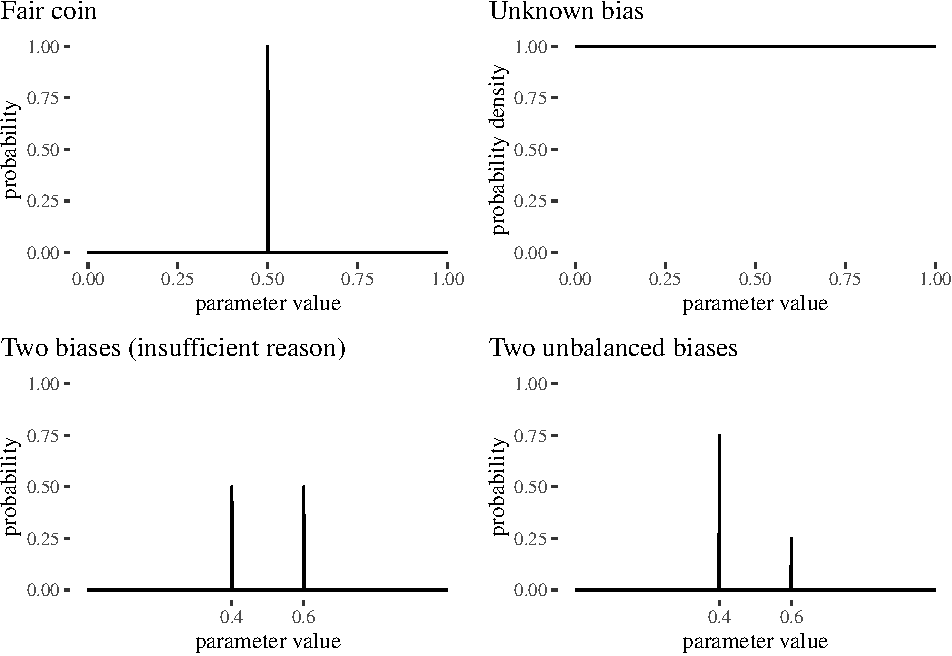
\includegraphics[width=1\linewidth]{chapter-outline_files/figure-latex/fig:evidenceResponse2-1} \end{center}
\caption{Examples of RA's distributions responding to various types of evidence for typical cases brought up in the literature.}
\label{fig:evidenceResponse}
\end{figure}

How is learning about frequencies modeled on this approach, assuming
independence and constant frequency/probability for all the
observations? The Bayes way. You start with some prior density \(p\)
over the parameter values. For instance, if you start with complete lack
of information, \(p\) might be uniform. Then you observe the data \(D\)
which is basically the number of successes \(s\) in a certain number of
observations \(n\). For each particular possible value \(\theta\) of the
parameter, the probability of \(D\) conditional on \(\theta\) follows
the binomial distribution. The probability of \(D\) is obtained by
integration. That is:

\begin{align*}
p(\theta \vert D) & = \frac{p(D\vert \theta)p(\theta)}{p(D)}\\
& = \frac{\theta^s (1-\theta)^{(n - s)}p(\theta)}{\int \theta'^s (1-\theta')^{(n - s)}p(\theta')\,\, d\theta'}
\end{align*}

For instance, belief inertia does not arise. If you just start with a
uniform density over \([0,1]\) as your prior, use binomial probability
as likelihood, observing any non-zero number of heads will exclude 0 and
observing any non-zero number of tails will exclude 1 from the basis of
the posterior, and the posterior distribution becomes more centered
around the parameter estimate as the observations come in. Let's see an
example with a grid approximation (\(n=1k\)) and coin tossing (grid
approximation allows us also to talk about probabilities rather than
densities). Our prior is uniform, and then, in subsequent steps, we
observe heads, another heads, and then tails. This is what happens with
the posterior as we go (Figure \ref{fig:intertia2}).

\begin{figure}[H]

\begin{center}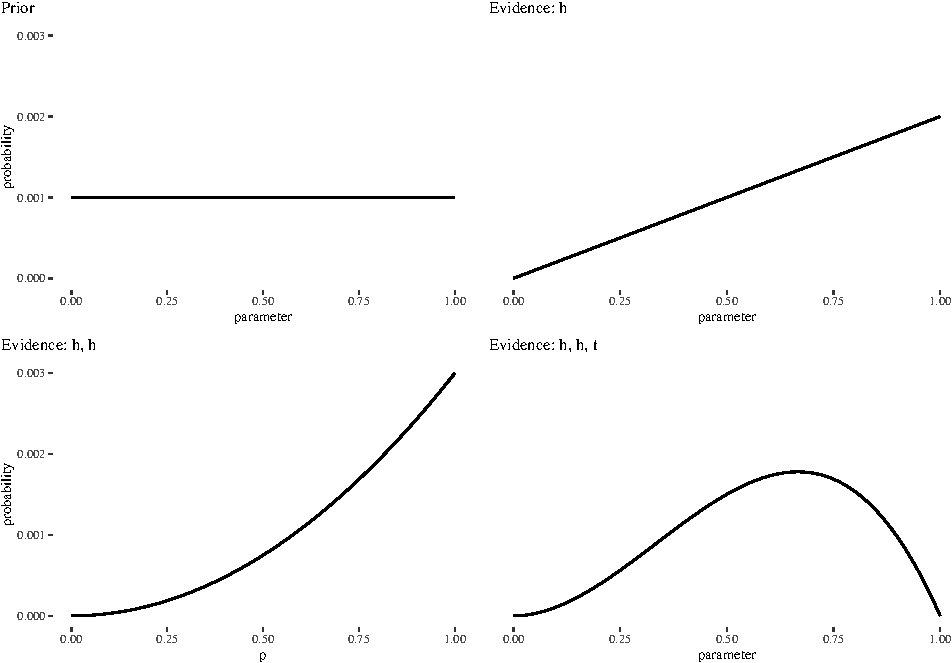
\includegraphics[width=1\linewidth]{chapter-outline_files/figure-latex/fig:inertia3-1} \end{center}
\caption{As observations of heads, heads and tails come in, extreme parameter values drop out of the picture and the posterior is shaped by the evidence.}
\label{fig:intertia2}
\end{figure}

\hypertarget{examples-of-applications}{%
\section{Examples of applications}\label{examples-of-applications}}

\hypertarget{adding-carpet-evidence-in-the-wayne-williams-case}{%
\subsection{Adding carpet evidence in the Wayne Williams
case}\label{adding-carpet-evidence-in-the-wayne-williams-case}}

\hypertarget{higher-order-probabilities-and-bayesian-networks}{%
\subsection{Higher-order probabilities and Bayesian
networks}\label{higher-order-probabilities-and-bayesian-networks}}

The reader might be worried: how can we handle the computational
complexity that comes with moving to higher-order probabilities? The
answer is, as long as we have decent ways of either basing densities on
sensible priors and data, or eliciting densities from experts (CITE
UNCERTAIN JUDMENTS), implementation is not computationally unfeasible,
as we can approximate densities using sampling. To illustrate, let us
start with a simplified BN developed by CITE FENTON to illustrate how
conviction was unjustified in the Clark case (Figure
\ref{fig:scBNplot}). to illustrate a point about the notorious Sally
Clark case (Figure \ref{fig:scBNplot}).\footnote{R. v. Clark (EWCA Crim
  54, 2000) is a classic example of how the lack of probabilistic
  independence between events can be easily overlooked. Sally Clark's
  first son died in 1996 soon after birth, and her second son died in
  similar circumstances a few years later in 1998. At trial, the
  paediatrician Roy Meadow testified that the probability that a child
  from such a family would die of Sudden Infant Death Syndrome (SIDS)
  was 1 in 8,543. Meadow calculated that therefore the probability of
  both children dying of SIDS was approximately 1 in 73 million. Sally
  Clark was convicted of murdering her infant sons (the conviction was
  ultimately reversed on appeal). The calculation illegitimately assumes
  independence, as the environmental or genetic factors may predispose a
  family to SIDS. The winning appeal was based on new evidence: signs of
  a potentially lethal disease---contrary to what was assumed in the
  original case---were found in one of the bodies.} The arrows depict
relationships of influence between variables. \textsf{Amurder} and
\textsf{Bmurder} are binary nodes corresponding to whether Sally Clark's
sons, call them A and B, were murdered. These influence whether signs of
disease (\textsf{Adisease} and \textsf{Bdisease}) and bruising
(\textsf{Abruising} and \textsf{Bbruising}) were present. Also, since
son A died first, whether A was murdered casts some light on the
probability of son B being murdered.

\begin{figure}[H]

\begin{center}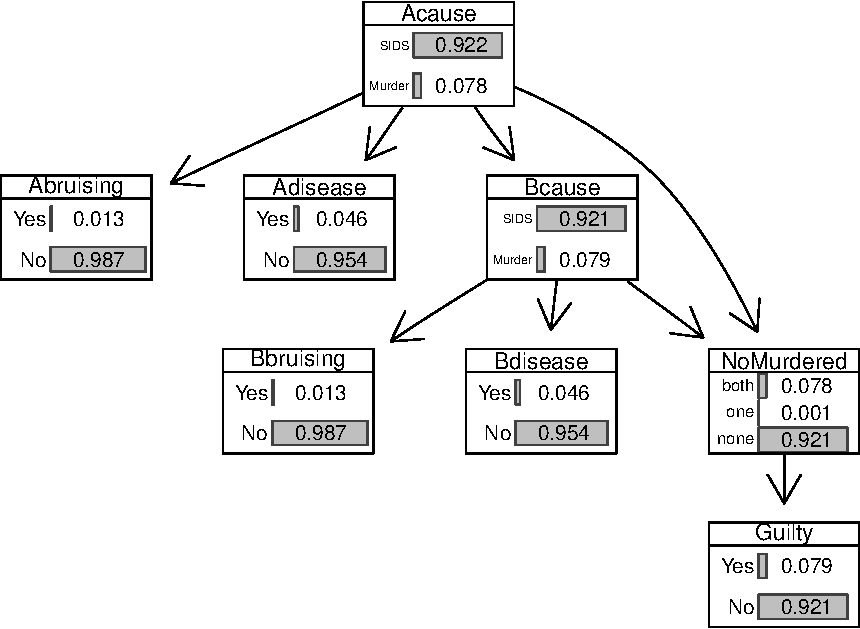
\includegraphics[width=0.8\linewidth]{chapter-outline_files/figure-latex/scBNplot2-1} \end{center}
\caption{The BN developed by FENTON ET AL., with marginal prior probabilities.}
\label{fig:scBNplot}
\end{figure}

The point to be illustrated was that with a sensible choice of
probabilities for the conditional probability tables in the BN,
conviction was not justified at any of the major stages (Figure
\ref{fig:SCfentonTable}).

\begin{figure}[H]

\begin{center}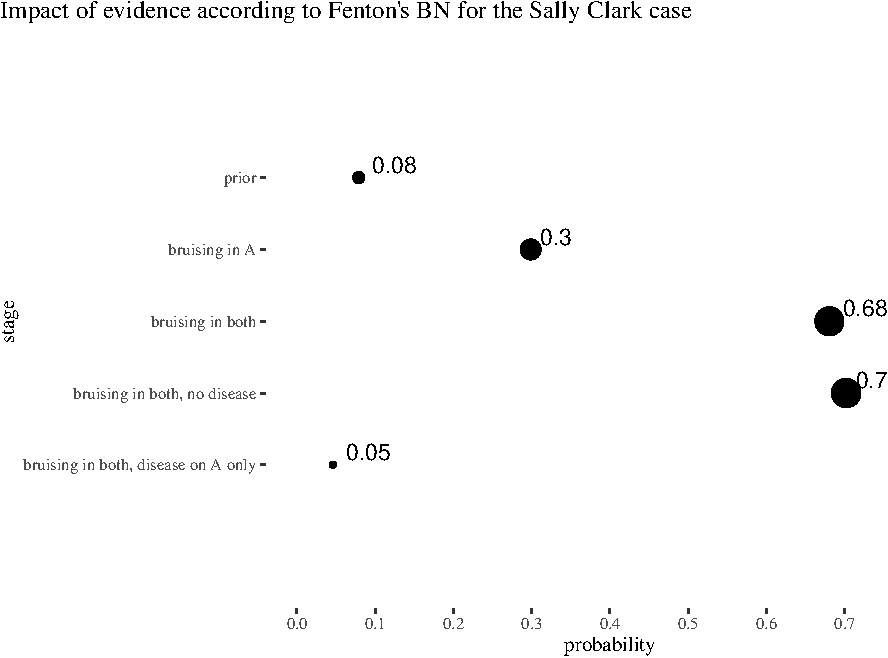
\includegraphics[width=1\linewidth]{chapter-outline_files/figure-latex/SCfentonTable2-1} \end{center}

\caption{The prior and posterior probabilities for Fenton's Sally Clark BN.}

\label{fig:SCfentonTable}

\end{figure}

One reason the reader might worry is that the choice of the
probabilities is fairly specific, and it is not obvious where such
precise values should come from. We have already discussed how frequency
and probability estimates usually come at least with some aleatory
uncertainty around them that cannot be represented by first-order
probabilities. The usual response REFS FOR SENSITIVITY ANALYSIS is that
a range of such selections should be tested, perhaps with special focus
on extreme but still plausible values. We have already discussed how
much care is needed on such approach as it to some extent ignores the
shape of the underlying distributions. Crucially, on the sensitivity
approach different probability measures (or point estimates) are not
distinguished in terms of their plausibility, and so this plausibility
is not accounted for in the analysis. Moreover, if in the sensitivity
analysis the further decision is guided by the results for the extreme
measures, they might play an undeservedly strong role. The best case
scenario for my way home from the office is that I find a suitcase with
a lot of money inside. The worst case scenario is that I get run over by
a bus. What is the quality of the guidance that the consideration of the
worst case and the best case scenario provide me with? Limited.

Some of these concerns are at least dampened when we deploy the higher
order probabilities in the BN. The general method is as follows. Each
particular node in a precise BN has a probability table determined by a
finite list of numbers. If it's a root node, its probability table is
determined by one number, if it's a node with one parent, its table is
determined by two numbers etc. Now, suppose that instead of precise
numbers we have densities over parameter values for those determining
numbers. Densities of interests can then be approximated by (1) sampling
parameter values from the specified distributions, (2) plugging them
into the construction of the BN, and (3) evaluating the probability of
interest in that precise BN. The list of the probabilities thus obtained
will approximate the density fo interest. In what follows we will work
with sample sizes of 10k. For instance, your conditional probabilities
might look as illustrated in Figure \ref{fig:SCwithHOPa}. One of them is
based on a truncated normal distribution to emphasize that the framework
give us much freedom in the specification of distributions.

\begin{figure}[H]

\begin{center}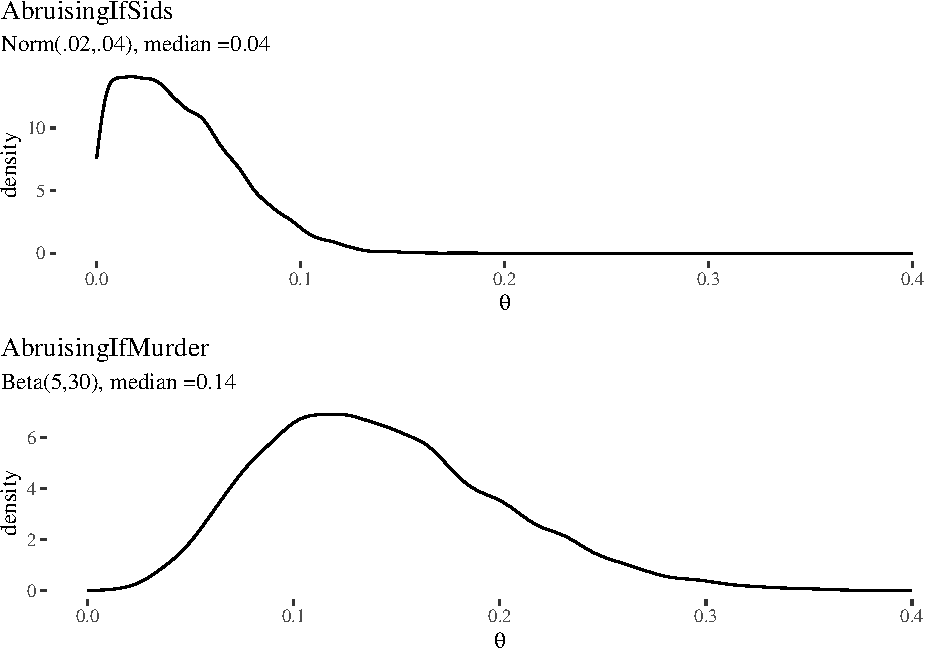
\includegraphics[width=0.9\linewidth]{chapter-outline_files/figure-latex/fig:SCwithHOPa-1} \end{center}
\caption{Example of approximated uncertainties about conditional probabilities in the Sally Clark case.}
\label{fig:SCwithHOPa}
\end{figure}

\begin{figure}[H]

\begin{center}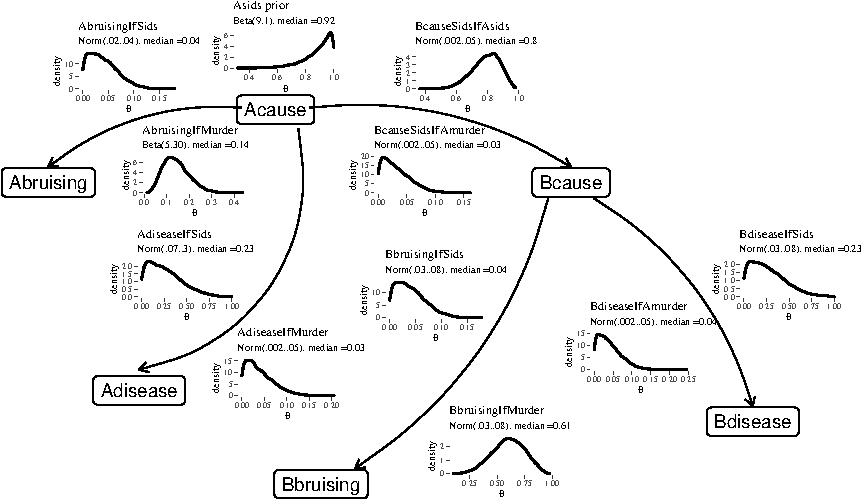
\includegraphics[width=1.6\linewidth,height=2\textheight,angle=90]{chapter-outline_files/figure-latex/SCwithHOP-1} \end{center}

\caption{Example of a HOP approach tor the Sally Clark Case  approximated by sampling probabilities  and constructing 10k BNs.}
\label{fig:SCwithHOP}
\end{figure}

Using these we can investigate the impact of incoming evidence as it
arrives (Figure \ref{fig:SCwithHOP2}). We start with the prior density
for the \s{Guilt} node. Then, we update with the evidence of signs of
bruising in both children. Next, we consider what would have happened if
also both children showed no sign of potentially lethal disease.
Finally, we look at the (simplified) evidential situation at the time of
the appeal: signs of bruising in both children, and signs of lethal
disease discovered in only the first child. One thing to notice that
even in the strongest scenario against Sally Clark (third
visualization), while the median of the posterior distribution was above
.95, the uncertainty around that median is still too wide to legitimize
conviction as the lower limit of the 89\% HPDI is at .83. This
illustrates the idea that taking the point estimates and running with
them might lead to overconfidence, and that paying attention to
uncertainties about the estimates can make an important difference to
our decisions and their accuracy.

\begin{figure}[H]

\begin{center}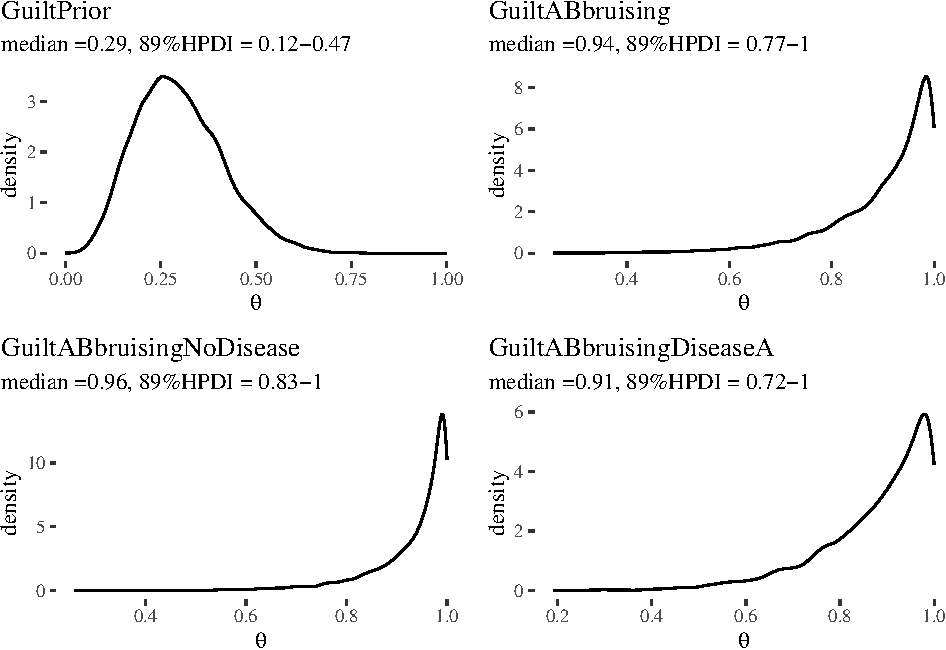
\includegraphics[width=0.9\linewidth]{chapter-outline_files/figure-latex/SCwithHOP2-1} \end{center}


\caption{Impact of incoming evidence in the Sally Clark case.}
\label{fig:SCwithHOP2}
\end{figure}

Moreover, if we are interested in likelihood ratios, the same approach
can be used: sample from the selected distribution appropriate for the
conditional probabilities at hand, then divide the corresponding
samples, obtaining a sample of likelihood ratios, approximating the
density capturing the recommended uncertainty about the likelihood
ratio. For instance, we can use this tool to gauge our uncertainty about
the likelihood ratios corresponding to the signs of bruising in son A
and the presence of the symptomps of a potentially lethal disease in son
A (Figure \ref{fig:SClrs}).

\begin{figure}[H]


\begin{center}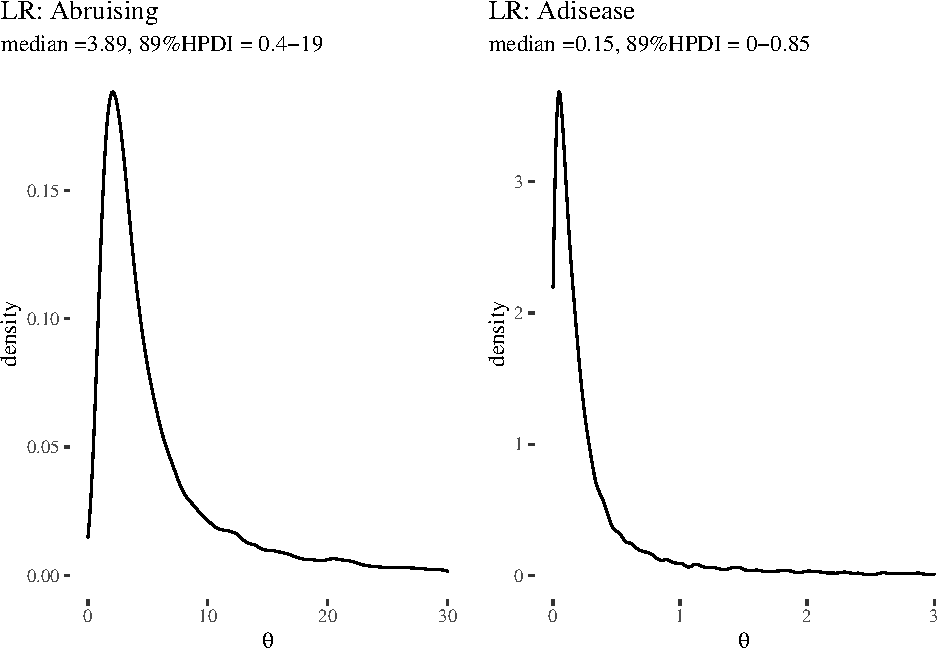
\includegraphics[width=0.9\linewidth]{chapter-outline_files/figure-latex/SClrs-1} \end{center}

\caption{Likelihood ratios forbruising and signs of disease in child A in the Sally Clark case.}
\label{fig:SClrs}

\end{figure}

\hypertarget{impact-of-false-positives-in-dna-identification}{%
\subsection{Impact of false positives in DNA
identification}\label{impact-of-false-positives-in-dna-identification}}

Let us get back to the problem we already discussed in Chapter 5: the
question of the extent to which the probability of a false positive
impacts the value of DNA match evidence. We already argued that the
probability of false positives is non-negligible. Here higher-order
probability will assist us in thinking through a comment in an important
paper on the topic (Thompson, Taroni, \& Aitken, 2003, p. 3):

\begin{quote}
If, as commentators have suggested, the rate of false positives is between 1 in 100 and 1 in 1000, or even less, then one might argue that the jury can safely rule out
the prospect that the reported match in their case is due to error and can proceed to consider the probability of a coincidental match. For reasons we will explain more fully below, this argument is fallacious and profoundly misleading \dots As we will explain below, the probability that a reported match occurred due to error in a particular case can be much higher, or lower, than the false positive probability. 
\end{quote}

One option would be to use these interval edges to investigate the
consequences of the risk of a false positive in DNA identification. But,
we hope to have already convinced the reader, the consequences of doing
so might be too skeptical, and it would be much better if we had a
sensible distribution to reason with.

Let us use Bayes' theorem again to think about false positives. This
time, instead of on likelihood ratios, we focus on posterior
probability. The posterior probability of the source hypothesis (\(S\))
conditional on the match evidence (\(E\)) is:

\begin{align*}
\pr{S \vert E} &   =  \frac{\pr{E\vert S} \pr{S} } {\pr{E}}\\
& = \frac{\overbrace{\pr{E\vert S}}^1 \pr{S}}{\underbrace{\pr{E\vert S}}_1 \pr{S} + \underbrace{\pr{E \vert RM}}_1 \pr{RM} + \underbrace{\pr{E \vert FP}}_1 \pr{FP}} \\ & = \frac{\pr{S}}{\pr{S} + \pr{RM} + \pr{FP}} 
\end{align*}

For simplicity we take the false negative rate to be zero, that is we
assume \(\pr{E\vert S} =1\). We also assume there are three ways the
evidence could arise: the source hypothesis is true, a random match
(\(RM\)) occurred, or we are dealing with a false positive (\(FP\)).

Now, let us start with calculations which ignore false positive risk and
take \(FP=0\). Suppose RMP is \(10e-9\) (as in some of the examples we
discussed in Chapter 5). The relation between priors and the posteriors
is illustrated with dashed orange line in Figure \ref{fig:fplinesPlot}
(to be explained fully later on), and the evidence seems quite strong:
the minimal prior sufficient for the posterior to be above .99 is 0.001.

Next, let us run charitable calculations with the upper edge of the
interval offered for \(FP\), 0.01. Then, the posterior of \(.99\) is
reached only once the prior is above .99, and the evidence seems rather
weak. So which is it? None. Running with the extreme scenario
over-appreciates and running with the point estimate under-appreciates
the uncertainty involved. What matters between the edges matters.

Consider two scenarios. In both you think that with 99\% certainty the
false positive rate is between 0.001 and 0.01. On one approach you think
that any value between these values (with a slight leeway on top) is
equally likely, while on the other you think that it is 50\% likely that
\(FP\) is below .0033. The latter distribution, while being centered
closer to zero has another features: it is long-tailed, so at the same
time you do not think that \(FP\)s above .01 are impossible---you allow
for the rare possibility of a false positive being much higher (say, if
some specific conditions or circumstances arise, but you have no
knowledge of how to identify them, because extensive studies on false
positives are only forthcoming), in line with the passage quoted above.
These distributions are illustrated in Figure \ref{fig:fppdistros}.

\begin{figure}[H]



\begin{center}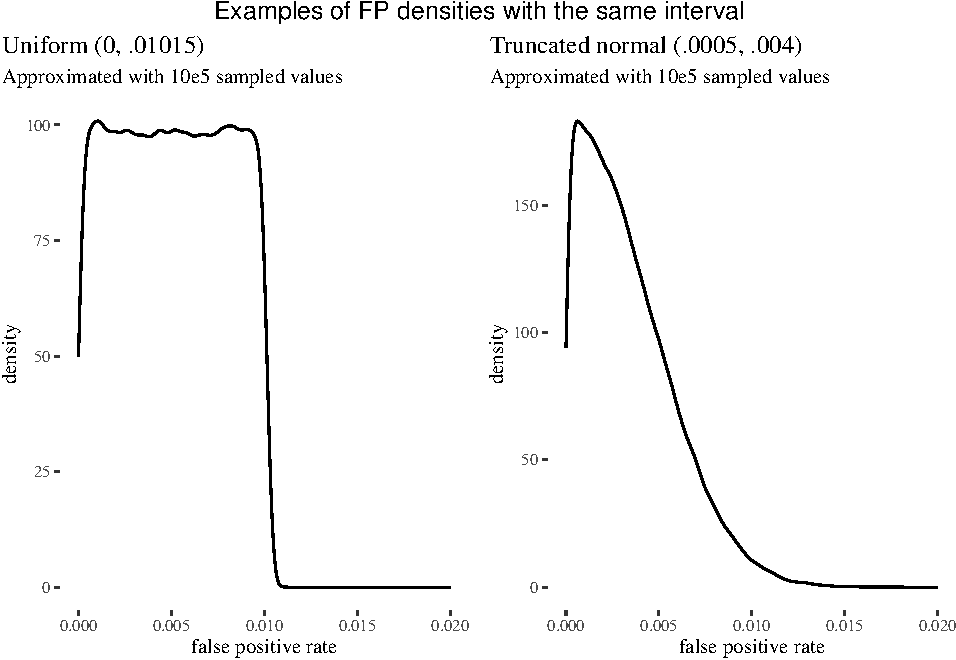
\includegraphics[width=0.8\linewidth]{chapter-outline_files/figure-latex/fig:fppdistros-1} \end{center}


\caption{Two examples of assumptions about the false positive rates, both having pretty much the same 99\% highest density intervals. (Top) all error rates are equally likely, (Bottom) the most likely values are closer to 0, but also some high values while unlikely are possible.}

\label{fig:fppdistros}

\end{figure}

Let us use sampling from the distributions to investigate what
differences arise depending on what one's second-order convictions about
error rates are. First, we ask what the distributions of minimal priors
sufficient for the posteriors being above .99 for these two options are
(if the minimum is 1 this means that no prior results in such a
posterior). The answer is illustrated in Figure \ref{fig:fppMinima}.

\begin{figure}[H]



\begin{center}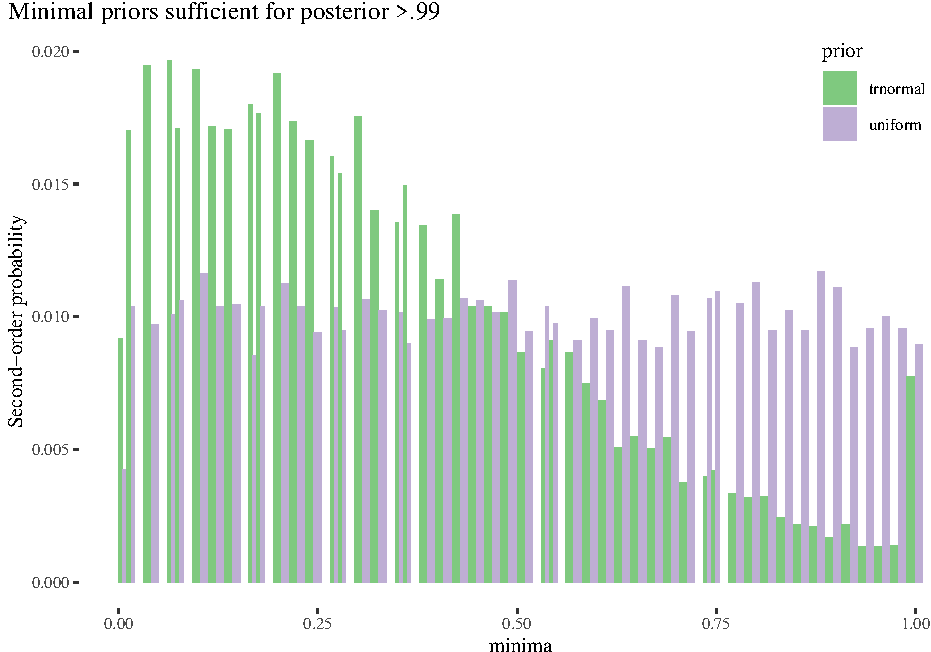
\includegraphics[width=0.8\linewidth]{chapter-outline_files/figure-latex/fig:fppMinima-1} \end{center}


\caption{The distribution of minimal priors sufficient for the posterior being above .99 on the two distributions of false positive rates. Note that the truncated normal distribution has its bulk towards the left, but at the same time has higher ratio of evens in which this posterior is never reached. }

\label{fig:fppMinima}

\end{figure}

Notice how the uniform distribution which seriously ``thinks'' that all
false positive rates in the interval are equally likely leads to highly
skeptical evaluation of the evidence. On both approaches the evidence is
insufficient for conviction, but 95\% of the minima on the truncated
normal distribution are below .8, whereas the 95th quantile for the
minima for the uniform distribution is rather unsurprisingly at .95.
That is, the truncated normal gives a more balanced and honest picture
that the charitable reading which runs only with one extreme value.

Another perspective on the impact of such differences can be taken by
inspecting a large number of lines (in our case, 300) of how the
posterior depends on the posterior: their density corresponds to the
density of the false positive rates. We illustrate these in Figure
\ref{fig:fplinesPlot}.

\begin{figure}[H]

\begin{center}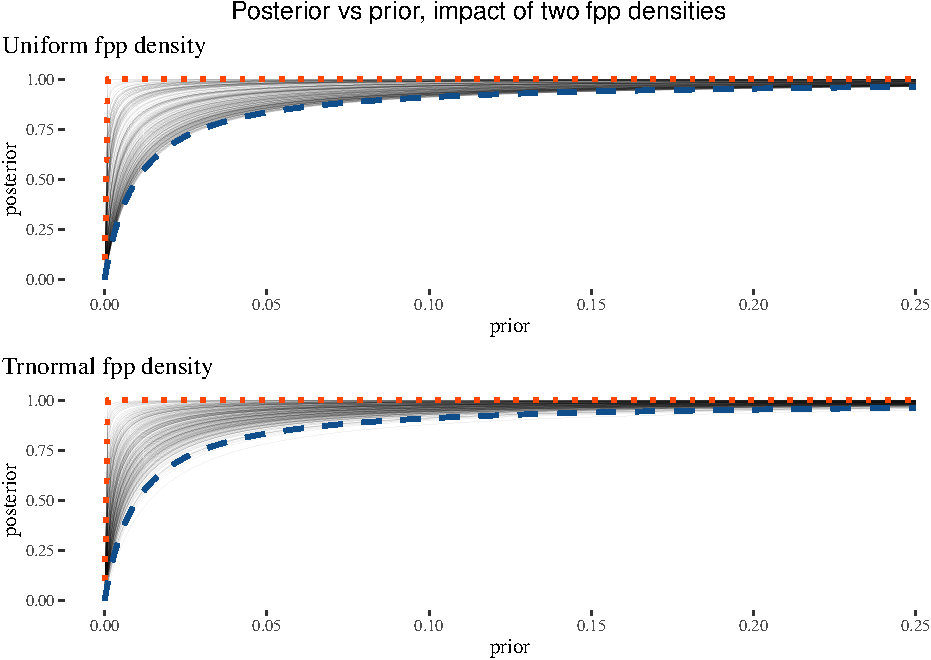
\includegraphics[width=0.8\linewidth]{chapter-outline_files/figure-latex/fig:fplinesPlot2-1} \end{center}
\caption{Impact of prior on the posterior assumign two different densitites for false positive rates. Note how both the "pristine" error-free point estimate (orange) and the charitable version (blue) are quite far from where the bulks of the distributions in fact are. Note also how the trnormal density allows for even more charitable cases, which results from it being long-tailed.}
\label{fig:fplinesPlot}
\end{figure}

Suppose now you indeed are convinced that the distribution over possible
false probability values indeed matters for the evaluation of DNA
evidence. But where do we take these distributions from, you might ask.
The problem is, studies on false positives are very limited and so only
give a rough and foggy picture. Ideally, better experiments and studies
which would allow for a better justification of the choice of a
distribution, should be conducted. However, this does not mean that
until then we should stick to using point estimates and interval edges.
Once the functional form of the distribution, such as truncated normal
or beta, which are known to be pretty standard and reliable in such
contexts, are chosen, only a few numbers need to be elicited from
experts to be able to construct a density. For instance, once we agree
on the truncated normal form, it is enough that the expert says that the
99\% interval is as the one we used, and that she believes with more
than 50\% confidence the false positive rates to be below \(.033\) for
the curve to be determined. There is, of course, some idealization
involved, and having to rely on such elicitation is not perfect. But it
is still better than asking the experts for single point estimates and
relying on these.

\pagebreak

\hypertarget{objections-to-the-higher-order-approach}{%
\section{Objections to the higher-order
approach}\label{objections-to-the-higher-order-approach}}

You might have some concerns about the way we propose to use
higher-order probabilities and densities in evidence evaluation. Some
prominent scholars in field certainly do. Taroni et al. (2015) argue
extensively for the experts reporting only point estimates, and their
objections deserve attention.

Their point of departure is a reflection on match evidence. The
prosecution hypothesis, \(H_p\) is that the suspect is the origin of the
trace, and the defense hypothesis, \(H_d\), is that another person,
unrelated to the suspect is the origin of the trace. The evidence \(E\)
is that a match has been reported. Typically, if \(H_p\) holds, it is
assumed the laboratory will report a match, so that
\(\pr{E\vert H_p}=1\) and the likelihood ratio reduces to
\(\nicefrac{1}{\pr{E \vert H_d}}\). This probability can be estimated on
the frequentist approach, on which probability is interpreted as the
limiting or population frequency \(\theta\), and an agent in fact does
estimate the true parameter in terms of a probabilistic distribution
\(p(\theta)\) over its possible values. For instance, in DNA evidence
evaluation the allelic relative frequency \(f\) of DNA matches found in
an available database is an estimate of the true frequency in a given
population of interest. If the observations are realizations of
independent and identically distributed Bernoulli trails given
\(\theta\), the expert's uncertainty about \(\theta\) can be captured as
\(\s{beta}(\alpha + s + 1 ,\beta + n - s)\), where \(s\) is the number
of observed successes, \(n\) the number of observations in the database
(1 is added to the first shape parameter to include the match with the
suspect), and \(\alpha\) and \(\beta\) capture the expert's priors.

However, they insist, in front of the fact-finders, the expert is
supposed to report their epistemic uncertainty, which is to be
understood according to the subjective interpretation. On this
interpretation, probabilities express an agent's epistemic attitude
towards a proposition, their uncertainty about its truth value. Such
probabilities, Taroni et al. (2015) insist, unlike frequencies, are not
states of nature, but states of mind associated with individuals. For
this reason, they claim, it makes no sense to talk about second-order
uncertainty about subjective probabilities, as there is no underlying
state of the nature to estimate. Further, they insist this also applies
to likelihood ratios:

\begin{quote}
\dots there is no meaningful state of nature equivalent for the likelihood ratio in its entirety, as it is given by a ratio of two conditional probabilities. [p. 12]
\end{quote}

\noindent In line with this perspectives, in the elicitation of
probabilities Taroni et al. (2015) recommend investigating an agent's
betting preferences, and that a proper elicitation of this form will
lead to a single number.\footnote{``Clearly, one can adjust the measure
  of belief of success in the reference gamble in such a way that one
  will be indifferent with respect to the truth of the event about which
  one needs to give one's probability. This understanding is
  fundamental, as it implies that probability is given by a single
  number. It may be hard to define, but that does not mean that
  probability does not exist in an individual's mind. One cannot
  logically have two different numbers because they would reflect
  different measures of belief.'' {[}p.~7{]}} \noindent Moreover, while
they claim that it is fine to use distributions to talk about chance,
they deny this possibility for personal uncertainty, under the threat of
infinite regress:

\begin{quote}
One can, in fact, have probabilities for events, or probabilities for propositions, but not probabilities of probabilities, otherwise one would have an infinite regression. [p. 8]
\end{quote}

\noindent Accordingly, Taroni et al. (2015) insist that given a
frequentist estimation of the probability of the evidence given the
defense hypothesis, \dots

\begin{quote}
\dots personal beliefs [\dots] can be computed as:
\begin{align*}\pr{E} & = \int_{\theta} \pr{E\vert \theta} \pr{\theta}\,\, d\theta \\
& =  \int_\theta  \theta \pr{\theta}\,\, d\theta
\end{align*}
\end{quote}

\noindent In particular, for the DNA match example, they advice that the
personal belief is the expected value of the \(\s{beta}\) distribution,
which reduces to \(\nicefrac{\alpha + s + 1}{\alpha + \beta +n + 1}\).
They claim that it satisfactorily expresses the posterior uncertainty
about \(\theta\), and that it is solely this probability that should be
used in the denominator in the calculation and reporting of the
likelihood ratio.

This criticism has been countered by Sjerps et al. (2015). One point
they raise is that the distinction between states of nature which can be
estimated and mental attitudes which are purely subjective and cannot be
in any meaningful way estimated is a bit too hasty. Once the background
information, the priors, the hypotheses and the evidence are specified,
the higher-order uncertainty about \(\theta\) follows from the
probability calculus, and it is by no means arbitrary to what extent
various potential values of \(\theta\) are supported by the evidence.

Moreover, in reporting only a single value, Sjerps et al. (2015) argue,
the expert refrains from providing the fact-finders with other
information about \(\theta\) which is reasonably supported by the data
and can have impact on the result of evidence evaluation and
incorporation. Crucially, the fact finders are interested in what Sjerps
et al. (2015) call the reliability of the evidence, and it depends on
the distribution (as we already illustrated in the first section of this
chapter). There is a difference between the expert being certain
\(\theta\) is \(.1\), their best estimate being .1 based on a thousand
of observations, an their best estimate being .1 based on ten
observations. Complete information about the impact of the evidential
basis of an estimate on expert's uncertainty about it allows the
fact-finders to reasonably go about trying to be on the safe side
working on the presumption of innocence.

To be fair, Taroni et al. (2015) at some point suggest that the expert,
aside of providing a point estimate, should also informally explain how
the estimate was arrived at, and that it would be helpful if the
recipients of this information were instructed in ``the nature of
probability, the importance of an understanding of it and its proper use
in dealing with uncertainty'' {[}p.~16{]}. But we think and our examples
illustrate that depriving non-expert fact finders of clearly
quantifiable information about aleatory uncertainty related to the
parameter of interest, replacing this information with an informal
description of what the expert did, while telling them that the nature
of probability is important and hoping for the best when it comes to
their proper assessment and use of the point estimates is wildly
optimistic, to say the least.

Dahlman \& Nordgaard (2022) criticize (Taroni et al., 2015) on more
philosophical grounds. Replying to the criticism based on probabilities
being legitimately assigned only to events, they use the betting
interpretation that the authors use themselves and push back, saying
that since a probability assessment is a betting preference, a
probability assessment is in itself an event: ``the formation of a
betting preference by a certain person at a certain time'' {[}p.~15{]}.
Replying to the infinite regress objection, they point out that
integrating higher order uncertainty does not a priori decrease the
first order probability and might as well increase it, so that going
higher-order does not in principle have to lead to skepticism. Finally,
their reply to the integration recommendation is somewhat case-specific,
as on their approach to the weight of evidence they deal with multiple
probability measures, and so their integration would be illegitimate.

Before we get into the surprisingly philosophical intricacies of the
debate between forensic scientists and legal evidence scholars, let us
make a point that should convince you that the higher-order approach is
preferable, no matter your philosophical convictions about the nature of
probability, propositions or the relation between uncertainty and
betting behavior. The point is simple. If you dump free information that
you already have in the densities and run with point estimates, your
predictions about the world will be less accurate in a very precise
quantifiable sense.

First, let us go over a particular example. We randomly draw a true
population frequency from the uniform distribution. In our particular
case, we obtained 0.632. Then we randomly draw a sample size as a
natural number between 10 and 20 (our points holds with larger samples,
just the discrepancies get smaller). In our particular case, it is 16.
Now we simulate an experiment in which we draw that number of
observations from the true distribution. In our particular case this
happened to lead to the observation of 8 successes. We use this number
to calculate the point estimate of the parameter, which is 0.5. Now we
ask about the probability mass function for all possible outcomes of an
observation of the same size. On one hand, we have the true probability
mass based on the true parameter. On the other, we have the probability
mass function based on the point estimate which is basically binomial
around the point estimate. On the third hand, we take the uncertainty
involved in our estimate of the parameter seriously, and so we first
take a sampling distribution of size 1e4 of possible parameter values
from the posterior
\(\s{beta}(1+\s{successes}, 1+\s{sample size} - \s{successes})\)
distribution (we assume uniform prior for the sake of an example). Then
we use this sample of parameter values to simulate observations, one
simulation for each parameter value in the sample. This results in the
so-called posterior predictive distribution, which instead of a point
estimate, propagated our uncertainty about the parameter value into our
predictions about the outcomes of possible observations. Then we take
simulated frequencies as our estimates of probabilities. This
distribution is more honest about uncertainty and wider than the one
obtained using the point estimate. All these are illustrated in Figure
\ref{fig:posteriorPrediction}.

\begin{figure}[H]

\begin{center}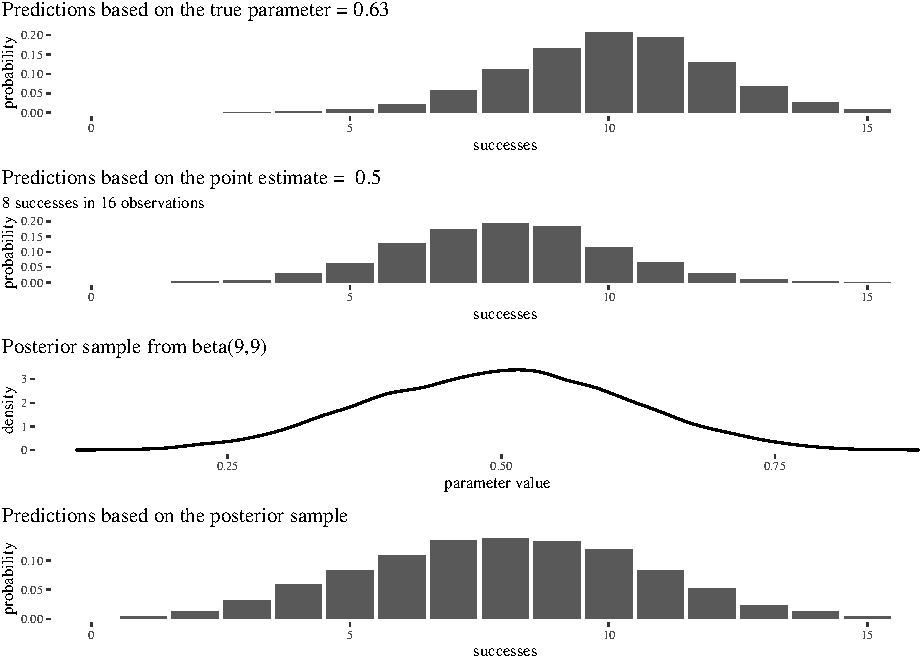
\includegraphics[width=0.9\linewidth]{chapter-outline_files/figure-latex/fig:posteriorPrediction2-1} \end{center}


\caption{Real probability mass, probability mass calculated using a point estimate, sampling distribution from the posterior, and the posterior predictive distribution based on this sampling distribution.}
\label{fig:posteriorPrediction}
\end{figure}

Notably, the PMF based on a point estimate is further off from the real
PMF than the posterior predictive distribution. For instance, if we ask
about the probability of the outcome being at least 9 successes, the
true answer is 0.7984, the point estimate PMF tells us it is 0.4056,
while the posterior predictive distribution gives a somewhat better
guess at 0.4277. Interestingly, a similar thing happens when we ask
about the probability of the outcome being at most 9 successes. The true
answer is 0.3681, the point-estimate-based answer is 0.778, while the
posterior predictive distribution yields 0.7051. More generally, we can
use Kullback-Leibler divergence to measure how far the point-estimate
PMF and the posterior predictive PMF are from the true PMF. In our
particular case, the former distance is 0.7905638 and the latter is
0.5681121. That is, the posterior predictive distribution is
information-theoretically closer to the true distribution.

Now let us see how this point holds generally. Let's repeat the whole
simulation 1000 times, each time with a new true parameter, a new sample
size, and a new sample. Every time we construct the PMFs using the
methods we described, and measure their KLD distances. Here is the
empirical distribution of the results of such a simulation (Figure
\ref{fig:kldsPlots})---we are looking at the differences in KLD
divergencies, positive differences mean the point-estimate based
distribution was further from the true PMF than the posterior predictive
PMF. Notably, the mean difference is 0.865, the median difference is
0.044, and the distribution is asymmetrical, as there are multiple cases
of huge differences favoring posterior predictive distributions. That
is, accuracy-wise, point-estimate-based PMFs are systematically worse
than posterior predictive PMFs.

\begin{figure}[H]

\begin{center}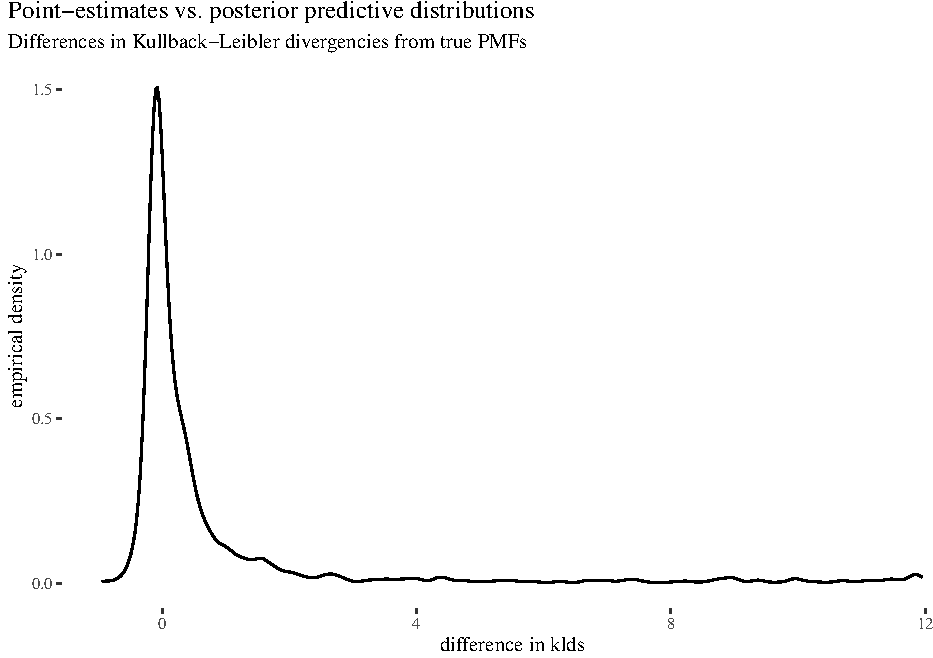
\includegraphics[width=0.9\linewidth]{chapter-outline_files/figure-latex/fig:kldsPlots-1} \end{center}
\caption{Differences in Kullback-Leibler divergencies from the true distributions, comparing the distributions obtained using point estimates and posterior predictive distributions. Positive values indicate the point-estimate-based PMF was further from the true distribution that its competitor.}
\label{fig:kldsPlots}
\end{figure}

If accuracy considerations do not convince you, we can also get more
philosophical. As the betting behavior interpretation is actually not as
obvious or uncontroversial as Taroni et al. (2015) suggest,\footnote{See
  philosophical textbooks on formal epistemology such as (D. Bradley,
  2015) or (Titelbaum, 2020).} we prefer to respond without assuming it,
just working with the assumption that an agent's probabilities or
densities are to represent or capture their uncertainty.

First, Taroni et al. (2015) seem to argue that since first-order
probabilities capture your uncertainty about a proposition of interest,
second-order probabilities are supposed to capture your uncertainty
about how uncertain you are, and that ``estimating'' your first-order
uncertainties would be a bit silly---after all, they seem to think, you
can simply figure out your fair odds in a related bet on the proposition
in question, and those would give you your unique first-order
uncertainty without any uncertainty about it.

There are more controversial claims that philosophers have argued for
than the infallibility of introspection. Those involved with epistemic
logic often argue that it is not even the case that if an agent knows
(or doesn't know) \(p\), they also automatically know that they (don't)
know \(k\). Analogously, it would not be a completely implausible
philosophical position to say that we sometimes are uncertain about what
we think the fair bets are or what our first-order uncertainties are.
This is one possible path of answering this.

But we think there is a better way. Let us think again about our expert,
who gathers information about the allelic relative frequency \(f\) of
DNA matches in an available database, and starts with some defensible
\s{beta} prior with parameters \(\alpha, \beta\). Say they observe \(s\)
matches and the database size is \(n\). They reach a
\(\s{beta}(\alpha + s + 1 ,\beta + n - s)\) distribution over the
possible RMP values. So far, nothing controversial happens---they are
estimating the relevant population frequency. Assuming the conditions
are pristine (the expert has no modeling uncertainty, does not have
consider la ab errors and so on),\footnote{Otherwise they need to think
  harder and dampen their convictions.} they want to use this
distribution to shape their subjective uncertainty. But uncertainty
about what? One obvious proposition is
\emph{a match is observed  if another person, unrelated to the suspect is the origin of the trace}.
And indeed, insofar as only this proposition is being considered, it is
yet not clear what second-order uncertainties would be uncertainties
about. But the expert also considers a continuum of propositions, each
of the form \emph{the true population frequency is $\theta$} for each
\(\theta\in [0,1]\). A density over \(\theta\) can be simply seen as
capturing the comparative plausibility that the expert assigns to such
propositions in light of the evidence, and normalization allows them to
calculate their subjective probabilities for \(\theta\) belonging to
various sub-intervals of \([0,1]\). So if you were worried that there
were no propositions that the expert could be ``second-order'' uncertain
about, the good news is, there are plenty. In particular, if \(\theta\)
is supposed to be a population frequency, gauging which density captures
the extent to which the evidence justifies various estimates of that
frequency is pretty much the same as gauging comparative plausibility of
the corresponding propositions about the population frequencies. Now,
you might complain that this should no longer be called ``estimation'',
but you might also think that the connection is strong enough to justify
this terminology. This is a verbal discussion that we will not get into,
language users' linguistic behavior will decide this for us anyway.

More generally, evidence justifies various first-order probability
assignments to varying extent. If we have no evidence about the bias of
a coin, each first-order uncertainty about it is equally (un)-justified
(if you like to think in terms of bets: the evidence gives us no reasons
to prefer any particular odds as fair). If we know the coin is fair, the
evidence clearly selects one preferred value, .5 (and, again, if you
like the betting metaphor, one preferred betting odds). But often the
evidence is stronger than the former and weaker than the latter
case---one clear example of this phenomenon is if we consider
propositions about population frequencies in light of the results of
observations---in such circumstances, the evidence justifies different
values of first-order uncertainty to varying degree, and densities
simply capture the extent to which different first-order uncertainties
are supported by the evidence. So what is it that you are estimating?
The ideal evidential support you would get if you had all the evidence.
Why is the estimate off? because your evidence is limited and the best
you can do is gauge your uncertainty going where this limited evidence
leads you.

What about the objection that these are not ``states of nature'' and so
cannot be estimated? We are not sure about ``nature'' and why the
requirement of being part of nature is important for estimation. We have
seen cases of mathematicians using approximate methods to estimate
answers to fairly abstract questions not obviously related to ``states
of nature'', whatever these are, and so we think estimation makes sense
whenever there are some objective answers that get closer or further
from. But if there is some objectivity to what the ideal evidence would
support, or to the extent to which the actual evidence supports various
competing hypotheses, we can be more or less wrong about such things,
and so it is not implausible to say that there is a clear sense in which
we can estimate them.

What about the threat of infinite regress? Surely, Taroni et al. (2015)
would agree that one can be uncertain about a statistical model. But
this can be the case even if this model spits out a point estimate
rather than a density. This would suggest that if you think the
possibility of putting uncertainty on top of propositions about possible
values of a first-order parameter leaves us in an epistemically hopeless
situation, you might have hard time explaining why your point estimation
is in a better situation. After all, if asking further questions about
probabilities up the hierarchy is always justified, we can keep asking
about the probability of a point-estimate-spitting model being adequate,
the probability of that probability (and the way we have reached it)
being adequate and so on. Alternatively, we could concede that while our
situation is often epistemically difficult, it is not hopeless. Of
course, the mathematical and statistical models we use are exactly
those: models, which can be more or less epistemically helpful. And when
we decide which models to use, we always face a trade-off between
various factors. In particular, second-order estimation is more complex
than running with point estimates. But by now we hope to have convinced
the reader this complexity is worth the effort. What about more complex
models going even higher? Well, if a case is made that there is a
workable approach that does that, which is worth the additional
complexity, we are all for it! In fact, some of the model selection
methods can be thought of this way. But to say that just because in
principle more complex models are always possible, we are facing some
sort of epistemic infinite regress is too hasty.

Finally, what about the idea that there is no ``meaningful state of
nature equivalent for the likelihood ratio in its entirety, as it is
given by a ratio of two conditional probabilities?'' If you think it is
meaningful to estimate two conditional probabilities (that is,
frequencies in the population), or to compare the relative plausibility
of various propositions about them in terms of density, it is equally
meaningful to estimate any function of the numbers involved. Otherwise
it would also be meaningless to try to estimate the BMI of an average 21
years old male student in the USA just because BMI is a ratio of other
quantities. There are various good reasons not to care about BMI too
much, but being a ratio of other numbers is not one of them.

\hypertarget{weight-of-evidence}{%
\section{Weight of evidence}\label{weight-of-evidence}}

We now illustrate one of the theoretical payoffs of higher-order
probabilism. It allows to develop an elegant theory of the weight of
evidence that outperforms existing proposals. We will start with an
informal sketch of the idea of the weight of evidence, as opposed to the
balance of the evidence. We will then explore a few attempts at modeling
this idea, first based on precise probabilism and then based on
imprecise probabilism. Finally, we will show how higher -order
probabilism can offer a better theory.

\hypertarget{motivating-examples}{%
\subsection{Motivating examples}\label{motivating-examples}}

In the 1872 manuscript \emph{The Fixation of Belief} (W3 295), C. S.
Peirce makes the following observation about sampling from a bag of
beans that are either black or white:

\begin{quote} When we have drawn a thousand times, if about half have been white, we have great confidence in this result ... a confidence which would be entirely wanting if, instead of sampling the bag by 1000 drawings, we had done so by only two.
\end{quote}

\noindent In both cases, our best assessment of the probability that the
next draw will be a black bean is .5, but how sure we should be of that
assessment is quite different depending on whether it is based on two or
one thousands draws. In other words, the \emph{weight} of the evidence
seems much greater after drawing 1,000 beans and finding out that half
are black, compared to drawing just two beans and again finding out that
half are black. The weight of the evidence is different in the two
cases, but its \emph{balance}---understood here as the relative
proportion of black-to-white beans---is the same.

Similar remarks can be found in Peirce's 1878
\emph{Probability of Induction}. There, he also proposes to represent
uncertainty by at least two numbers, the first depending on the inferred
probability, and the second measuring the amount of knowledge obtained.
For the latter, Peirce proposes to use some dispersion-related measure
of error (but then suggests that an error of that estimate should also
be estimated and so on, so that ideally more numbers representing errors
would be needed).

Peirce did not use the expression the weight of evidence (and, in fact,
he used the phrase to refer to the balance of evidence, W3 294) {[}CITE
KASSER 2015{]}. However, his remarks anticipated what came to be called
weight of evidence by Keynes in his 1921
\emph{A Treatise on Probability}:

\begin{quote}
As the relevant evidence at our disposal increases, the magnitude of the
probability of the argument may either increase or decrease, according as the new knowledge strengthens the unfavourable or the favourable evidence; but something seems to have increased in either case---we have a more substantial basis upon which to rest our conclusion. I express this by saying that an accession of new evidence increases the weight of an argument. (p. 71)
\end{quote}

\noindent The key point is the same {[}CITE LEVI 2001{]}: since the
balance of probability alone cannot characterize all important aspects
of evidential appraisal, another dimension---the weight of an
argument---must be deployed to quantify uncertainty.

Keynes entertained the possibility of measuring weight of evidence in
terms of the variance of the posterior distribution of a certain
parameter, but was quite attached to the idea that weight should
increase with new information, even if the dispersion may increase with
new evidence {[}TP 80-82{]}. So he proposed only a very rough sketch of
a positive proposal. Moreover, he was unclear how a measure of weight
could be part of decision-making. He was ultimately skeptical about the
practical significance of the notion. {[}TP 83{]}

\hypertarget{monotonicity}{%
\subsection{Monotonicity?}\label{monotonicity}}

It is instructive to examine more closely Keynes' claim that the weight
of evidence, unlike its balance, always increases as more evidence is
taken into account. While balance can oscillate one direction or the
other, weight would seem to always increase. We can state this
requirement as follows:

\begin{tabular}{lp{11cm}}
(Monotonicity) & If $E$ is relevant to $X$ given $K$, where $K$ is background knowledge, $V(X\vert K \wedge E) > V(X\vert K)$, where $V$ is the weight of evidence.
\end{tabular}

\noindent Monotonicity is corroborated by Peirce's example about drawing
from a bag of beans. As the sample size increases and the relative
proportion of black-to-white beans remains constant, the weight of the
evidence increases. That is:

\begin{tabular}{lp{11cm}}
(Weak increase) & In urn-like cases, the evidential weight obtained by a larger sample is greater, if the relative frequencies in the samples remain the same.
\end{tabular}

\noindent This formulation can be strengthened by dropping the
assumption of equal relative frequencies:

\begin{tabular}{lp{11cm}}
(Strong increase) & In urn-like cases, the evidential weight obtained by a larger sample is higher.
\end{tabular}

\noindent We think there are good reasons to reject Monotonicity and
Strong Increase, but we agree with Weak Increase. Monotonicity and
Strong Increase are consistent with a certain conception of the weight
of evidence, what we might call \emph{quantity} of evidence. After all,
there is no doubt that, as more evidence is taken into account, the
quantity of the evidence must increase. But the weight of evidence need
not be identified with its quantity alone. As more evidence is taken
into account, the new evidence may speak less clearly in favor or
against a hypothesis. For consider this example:

\begin{quote}
\textbf{A (possibly) rigged lottery:} Initially, you think the lottery  is  fair. You have no reason to doubt that. So, you calculate precisely the probability that a certain ticket number will be drawn. Then, rumors begin to surface that the lottery is rigged and that only numbers that satisfy a complicated equation will be drawn. You now have more relevant evidence at your disposal, but that evidence is more confusing and muddled than before. 
\end{quote}

\noindent Arguably, this is a scenario in which the quantity of evidence
has increased, but the weight of evidence has not. If this is right,
weight and quantity can come apart.

So, we seek a theory of evidential weight that can model two intuitions.
The first is that, as the sample size increases, the weight of the
evidence must also increase (under certain conditions, along the lines
of Weak Increase). The second intuition is that that, even when the
quantity of evidence increases, the weight of evidence might not (as
illustrated by the example of the rigged lottery).

\hypertarget{weight-and-precise-probabilism}{%
\subsection{Weight and precise
probabilism}\label{weight-and-precise-probabilism}}

An obvious place to look for a theory of the weight of evidence is
within precise probabilism. Without aiming to be exhaustive, we will
argue that our best bet is to look beyond precise probabilism.

\hypertarget{absolute-value-of-the-likelihood-ratio}{%
\subsubsection{Absolute value of the likelihood
ratio}\label{absolute-value-of-the-likelihood-ratio}}

The first attempt is a generalization of the likelihood ratio as a
measure of the value (or strength) of a piece of evidence relative to a
pair of competing hypotheses. Crucially, the likelihood ratio is a
\emph{directional} measure: the evidence may be favorable or unfavorable
to a hypothesis (compared to another). By contrast, Keynes' remarks
suggests that weight of evidence is a non-directional measure. It always
increases no matter the balance. To strip the likelihood ratio of its
directionality, it is enough to take the absolute value of the natural
log.
\todo{CITE: Nance's book "The Burdens of Proof" section 3.5. The quantification of Keynesian Weight.}
The weight of evidence \(E\) relative to the pair of hypotheses
\(H, H'\) would be \[\vert \ln (LR_{H, H'}(E)) \vert, \] where
\(LR_{H, H'}(E)=\frac{P(E \vert H)}{P(E \vert H')}\). By the properties
of logarithms, \(ln(1/x) = -ln(x)\), so two items of evidence of
equivalent strength---but opposite directionality---would have the same
weight. So, for example, \(|ln(1/3)|= |ln(3)| = 1.61\).

This account is simple and elegant, but faces two difficulties. The
first is technical in nature. As many have pointed out, there is a
problem with decomposition. Consider two items of evidence that, taken
together, have a likelihood ratio of one, say one has a likelihood ratio
of 1/3 and the other of 3. Assuming they are probabilistically
independent given a hypothesis of interest, their combined likelihood
ratio results from multiplying the individual likelihood ratios. Thus,
their combined weight would be zero since
\(\ln (LR_H(E1 \wedge E_2))=0\). However, by adding the weights one by
one, the combined weight would be different from zero, since
\(|ln(1/3)| + |ln(3)| = 3.22\). So, do the two items of evidence have
zero weight or not? Depending on how evidence is decomposed, it appears
to have different weights.

There might be a technical fix to the problem of decomposition. But
another, conceptually deeper problem exists. Whether the log of the
likelihood has a positive or negative sign, its absolute value is always
positive. Therefore, as more evidence is added, the weight of evidence
would always increase. This shows that this account agrees with
Monotonicity and Strong Increase, and in this sense, it only captures
the notion of quantity of evidence. The problem, then, is that it cannot
capture the intuition underlying the scenario of the rigged lottery in
which, even when quantity increases, weight does not.

\hypertarget{completeness-and-resilience}{%
\subsubsection{Completeness and
resilience}\label{completeness-and-resilience}}

Another strategy, within precise probabilism, is to model notions that
are related, albeit not identical, to weight. The literature has
suggested that precise probabilism contains the conceptual resources to
model two related ideas: resilience (or stability) and completeness.

Consider completeness first. \todo{CITE KAYE} Roughly, the proposal is
this: whenever the evidence available is missing information that one
would reasonably expect to see in a case, this fact must be taken into
account in assessing the probability of the hypothesis of interest. So,
instead of merely assessing \(P(H \vert E)\), one should assess
\(P(H \vert E \wedge M)\), where \(M\) is the known fact that some
evidence is missing. On this proposal, the missing evidence is not a
higher-order fact about the currently available evidence, but itself a
fact that counts as evidence together with other facts.

A good account of completeness should address a number of questions. For
example, under what circumstances, should an item of evidence count as
missing? Admittedly, there are cases in which it is clear that evidence
is missing, say because it was destroyed, lost or could not be retrieved
or collected for one reason or another. But evidence could be missing in
a more speculative sense. For example, if it is routine to see
breathalyzer evidence in drunk driving cases, what should one make of
the fact that such evidence is missing in a given case?\footnote{The
  more general worry here is that evidence is always incomplete.
  Peirce's example of drawing from a bag of beans makes this clear. In
  principle, more draws could be made and more evidence could be
  gathered.} Another difficulty concerns the impact that the missing
evidence should have on the other evidence. For example, in a case of
tax fraud, suppose the recording of phone conversation was deleted by
accident. There is no dispute about that. Now, should this fact increase
or decrease the probability that the defendant committed fraud?

Turn to resilience now. A precise probability assessment of \(H\) based
on some evidence \(E\), say \(P(H \vert E)\), is resilient (or stable)
whenever it does not wiggle too much relative to a reasonable set of
additional items of evidence \(E'\) that can be conditioned on. In other
words, \(P(H \vert E)\) is \emph{resilient enough} if and only if the
absolute difference \(| P(H | E) - P(H \vert E \wedge E')|\) (for any
element \(E'\) of a reasonable set of additional evidence) is within a
certain acceptable limit.\todo{CITE SKYRMS}

Resilience consists in evaluating a probability based on evidence not
yet available. The evidence could take different values---for example,
in a criminal case, the additional evidence could be exculpatory or
incriminating. How can additional evidence whose value is unknown affect
one's assessment of the probability of a hypothesis? Another question is
which further items of evidence should be included is the reasonable
set. Obviously, that set must be restricted somehow, or else no
probability assessment would ever be resilient. A good account of
resilience should address these questions.

Both resilience and completeness plays a role in trials proceedings. On
appeal, a defendant might argue that, had additional evidence be taken
into account, the verdict would have been different. Questions of
missing evidence are also routinely brought up in litigation. And the
rules of evidence often deal with questions of missing evidence and
offer a variety of remedies, from jury instructions to sanctions. In
this sense, a good theory of how evidence is assessed at trial should
include an account of completeness and resilience.

Suppose for now that attempts at formalizing resilience and completeness
can be successful---and we think they can be. A question remains,
however. Are resilience and completeness the theory of weight we are
looking for? This is far from clear. We conjecture that weight,
completeness and resilience are conceptually distinct notions and also
play distinct roles in legal fact-finding. So it is best not to conflate
them. Or at any rate, before identifying one with other, a good account
of each is needed. We sketch a few ideas about these three notions
towards the end.

\hypertarget{weight-and-imprecise-probabilism}{%
\subsection{Weight and imprecise
probabilism}\label{weight-and-imprecise-probabilism}}

A theory of weight can also be formulated using the conceptual resources
of imprecise probabilism. Unlike resilience and completeness, this
theory aims to model weight upfront.
\todo{CITE WEATHERSON ON WEIGHT AND IMPRECISE PROBABILISM} The idea is
this: a body of evidence is weightier whenever the representor set of
probability measures compatible with the evidence is smaller. Consider a
case of complete ignorance about the bias of a coin. The representor set
will contain \emph{any} probability measure. This corresponds to
complete lack of evidence and null weight, as expected. At the other
extreme, consider a case in which the fairness of the coin is known for
sure. The supporting evidence here would have maximal weight and the
representor set would only contain the precise probability measure that
assigns .5 to the two outcomes. All other intermediate cases would fall
somewhere in between.\footnote{More formally, let \(x_1\) and \(x_2\)
  the two extreme probability assignments in the representator set
  compatible with the available evidence \(E\). Then, the weight of
  \(E\) would be 1-\(x_1-x_2\). As expected, if there is only one
  probability measure, the weight would be one.}

This account accommodates the intuition underlying the rigged lottery
example. As more evidenced is accumulated, the representor set can
become larger and include more probability measures than before. Thus,
weight of evidence can decrease even when the quantity of evidence
increases. For this reason, a theory of weight based on imprecise
probabilism is promising. Its shortcoming, however, is that it inherits
the difficulties of imprecise probabilism, which we have already
mentioned. For example, recall that imprecise probabilism cannot model a
situation in which an epistemic agent believes that the coin could
biased .8 or .4, but thinks that one biased in more likely than the
other. Arguably, evidence compatible with the coin having two equally
likely biases should possess different weight than evidence compatible
with the coin having two biases one more likely than the other. The
latter situation is closer to full weight---the situation in which the
exact bias of the coin is known for sure. A theory of weight based on
imprecise probabilism is ill-equipped to accommodate these nuances.

\hypertarget{weight-and-higher-order-probabilism}{%
\subsection{Weight and higher order
probabilism}\label{weight-and-higher-order-probabilism}}

We are finally ready to present our own account of the weight of
evidence. This accout has two distinctive features. First, it is based
on higher-order probabilism. Second, it is information-theoretic. To
develop this account, we will begin with a sketch of Shannon's theory of
information.

\hypertarget{entropy-of-a-distribution}{%
\subsubsection{Entropy of a
distribution}\label{entropy-of-a-distribution}}

Let \(X\) be a random variable and \(P\) a probability distribution over
its values. Shannon's measure of information, \(H(X)\), reads:
\begin{align*}
H(X)  & =
- \sum \mathsf{P}(x_i) \log_2 \mathsf{P}(x_i)
\end{align*} \noindent  Consider the simple case in which \(X\) can take
two values---outcome 1 and outcome 0---whose probabilities are \(p\) and
\(1-p\). Figure (\textbf{REFER TO PLOT of H(X)}) shows \(H(X)\) as a
function of \(p\). As is apparent from the graph, \(H(X)\) is greatest
when the two outcomes have an equal probability of .5. The more the
probabilities deviate from .5, the more \(H(X)\) approaches zero.

To make sense of this, \(H(X)\) can be thought as the \textit{entropy}
(i.e.~the lack of information) contained in the distribution associated
with random variable \(X\). When the two outcomes have equal
probability, entropy is greatest. When they have different
probabilities, one outcome will be more probable than the other. The
more probable one of the outcomes (and thus the less likely the other),
the lower the entropy. Intuitively, \(H(X)\) captures the idea that
entropy is greatest when the indecision about which outcome will occur
is maximal, and the entropy decreases when such indecision decreases.

If \(H(X)\) is a measure of entropy---that is, a measure of lack of
information---why call it a measure of information? \(H(X)\) is also a
measure of information in the following sense: it describes the
\textit{expected amount of information} one would receive upon learning
the actual value of \(X\). After all, the higher the entropy, the less
informative a distribution, the more you expect to learn upon finding
out the actual value of \(X\). Conversely, the lower the entropy of the
distribution, the more informative the distribution, the less one
expects to learn upon finding out the actual value of \(X\).\footnote{Since
  working with continuous distributions is not straightforward, we will
  be using \emph{grid approximations} of continuous distributions: we
  will split \(X\) into a 1000 bins and use the normalized densities for
  their centers to obtain their corresponding probabilities. As long as
  we do not change our level of precision (which would inevitably lead
  to changes in entropy) in our comparisons, this is not a problem. An
  additional advantage is that now we do not have to deal with the
  intricacies of explicit analytic calculations for continuous
  variables.}

\hypertarget{informativeness-of-a-distribution}{%
\subsubsection{Informativeness of a
distribution}\label{informativeness-of-a-distribution}}

Since \(H(X)\) can be thought as the entropy of a distribution, we will
switch to the notation \(H(P)\). This notation emphasizes the
distribution \(P\) rather than the random variable \(X\). The entropy of
a distribution is to be contrasted with its informativeness, which we
will denote by \(W(P)\), the weight of the distribution. How should we
measure the informativeness (or weight) of a distribution?

Since informativeness is the opposite of entropy, it is tempting to take
the short route and define \(W(P)\) as \(1-H(P)\). But, for reasons that
will be become clear (\textbf{WHEN?}), the weight (or informativeness)
of a distribution is more aptly modeled by comparing it to the least
informative distribution, the uniform distribution which expresses
complete uncertainty. The idea is this: the more informative a
distribution, the more it departs from the uniform distribution, the
more weight it has, on a scale from 0 to 1. If the drop from uncertainty
is complete, the entropy drops to zero, and thus the weight should be 1;
if the drop is null, the entropy remains the same, and thus the weight
should be zero; if the drop is half, the weight should be .5; and so on
for other intermediate cases. This pattern can be captured by the
following definition of informativeness (or weight) of a distribution:
\begin{align*}
\mathsf{w(P_i)} & = 1 - \left( \frac{H(\mathsf{P})}{H(\mathsf{uniform})}\right)
\end{align*} \noindent where \(\mathsf{P}\) is the probability
distribution of interest and \(\mathsf{uniform}\) is the baseline
uniform distribution.\footnote{Since we are using grip approximation,
  \(\mathsf{P}\) is the discrete probability distribution for a given
  number of bins \(n\), and uniform is the discrete uniform distribution
  for the same number of bins. In some contexts it might make sense to
  measure improvement with respect to a non-uniform prior. In such
  cases, \(H(\mathsf{uniform})\) is to be replaced by
  \(H(\mathsf{prior})\). Note that the entropy of a uniform distribution
  is pretty straightforward, so we can simplify: \begin{align*}
  H(\mathsf{uniform}) & = \sum_{i=1}^n \nicefrac{1}{n} \log_2 \frac{1}{\nicefrac{1}{n}} \\
  & = \log_2(n) \\
  \mathsf{w(P_i)} & = 1 - \left( \frac{H(\mathsf{P})}{\log_2(n)}\right)
  \end{align*}}

The behavior of the proposed measure of weight can be illustrated using
distributions of various of shapes, displayed in Figure
\ref{fig:weightsWeird}). A bimodal normal distribution ``glued'' from
two normal distributions carries less weight than a unimodal normal
distribution with the same standard deviation centered around the mean
of the two modes. If multiple points have non-zero probability, the
weight depends on how uneven the distribution is. If the distribution
falls entirely on a single point, the weight is maximal (=1), as
expected.

\begin{figure}[H]

DISPLAY GRAPHS WITH DISTR OF VARIOUS SHAPES AND WEIGHT

\caption{Examples of various distributions with their entropies and weights, ordered by weights. (1) beta(4,4), (2) uniform starting from .5 to 1, (3), uniform strating from .6 to 1, (4) two normal distributions centered around .4 and .6 with standard deviation .05, glued at .5. (5) normal centered around .5 with the same standard deviation, (6) one that assigns .5 to each of .4  and .6, (7) One that assigns .3 to .4 and .7 to .6., (8) one that assigns all weight to .5, and (9) one that assigns all weight to .7.}

\label{fig:weightsWeird}
\end{figure}

\hypertarget{weight-of-evidence-1}{%
\subsubsection{Weight of evidence}\label{weight-of-evidence-1}}

Suppose a distribution \(P\) depicts what an agent thinks, at some point
in time, about the probability of the possible outcomes a random
variable \(H\). In this sense, the informativeness (or weight) of a
distribution \(W(P)\) measures how informed an agent is about \(H\). But
it measures the information level of an agent only relative to the state
of full uncertainty represented by the uniform distribution. There are
two things missing from this account: first, not every agent starts with
a uniform prior; second, how informed an agent is must depend on the
evidence available to that agent. What we need, then, is an account of
how informed agents are \textit{on the basis of the evidence} they have,
or in other words, an account of the weight (or informativeness) of the
evidence they have.

If the agent starts with a uniform prior over the values of a random
variable of interest, \(W(P)\) would be a good enough approximation of
how informed the evidence made them. In general, however, how much more
information is obtained is context-dependent. The weight of evidence,
then, must depend on what the agent already knows. Here is a general
recipe. In a given context, consider the prior distribution \(P_0\) for
the target hypothesis \(H\) given what the agent already knows. Then,
the agent updates by a body of evidence \(E\). Call this posterior
distribution \(P_E\), where the updating is done by standard Bayesian
conditionalization. Take the difference between the weight of the prior
distribution, \(W(P_0)\), and the weight of the posterior distribution,
\(W(P_E)\). The difference between the two--\(W(P_E)-W(P_0)\) or more
succinctly \(\Delta W\)---masures the impact that evidence \(E\) has on
the information level of the evidence. The difference \(\Delta W\),
then, is our proposed measure of the weight of the evidence.\footnote{If
  you prefer to think that weight of evidence should be always positive
  as a result of adding evidence, you might prefer the absolute value of
  the difference. We, however, prefer to keep track of whether the
  evidence makes the agent more or less informed about an issue.}

More precisely, the calculation follows the following schema:

\begin{enumerate}
\item Start with a prior distribution over the parameter space of interest and with distributions expressing the agent's uncertainty about other probabilities involved in the calculation of the posterior, say the likelihood of the evidence under different possible outcomes.
\item Sample from these distributions.
\item For each sample, treat it as a selection of precise probabilities, apply Bayes' theorem to calculate the posterior.
\item The set of the results is the sampling distribution expressing your posterior uncertainty.
\end{enumerate}

Higher order probabilism is then put to use to deliver a theory of
weight. What is now in \textbf{section 11} (``Weight of a
distribution'') and \textbf{sections 13} and \textbf{14} ('' Weight of
evidence'' and ``Weights in Bayesian Networks'') forms the bulk of the
theory.

We should also demonstrate that the proposed theory of weight does meet
the intuitive desiderata and can handle the motivating examples. To
better appreciset the novelty of the proposal, It might be interesting
to raise the following questions:

\begin{itemize}

\item[q1] what does a theory of weight based on precise probabilism look like? (maybe it consists of something like Skyrms' resilience or Kaye's completeness, the problem being that these are not measures of weight, but of something else, more on these later)

\item[q2] what does a theory of weight based on imprecise probabilism look like? (is Joyce's theory essentially an attempt to use imprecise probabilism to construct a theory of weight? )\todo{Well, it's a bit funny as Joyce's weight uses precise chance hypotheses instead of IP, so hard to say}

\item[q3] what does a theory of weight based on higher order probabilism look like?

\end{itemize}

Here we are defending a theory fo weight based on higher order
probabilism, but it is interesting to contrast it with a theory of
weight based on the other version of legal probabilism. Here we can also
show why Joyce's theory of weight does not work (either in the main text
or a footnote).

\textbf{Comment:} The current exposition in chapter 11, 13 and 14,
however, is complicated---perhaps overly so. The move from ``weight of a
distribution'' to ``weight of evidence'' is not intuitive and can
confuse the reader. Is there a simpler story to be told here? I think
so. See below.
\todo{Brilliant, I think I can start talking about conditional probabilities to begin with}

\textbf{Suggestion:} There seems to be a nice symmetry. Start with
precise probabilism. We can use sharp probability theory to offer a
theory of the value of the evidence (i.e.~likelihood ratio). Actually, I
think that the likelihood ratio model the idea of balance of the
evidence. What Keynes distinction weight/balance shows is that
likelihood ratio are not, by themselves, enough to model the value of
the evidence. The straightforward move here seems to just have
\textbf{higher order likelihood ratios}. Wouldn't higher order
likelihood ratio be essentially your formal model of the weight of the
evidence? Your measure of weight tracks the difference between (the
weight of the) prior distribution (and the weight of the) posterior
distribution. But higher order likelihood ratios essentially do the same
thing, just like precise likelihood ratios track the difference between
prior and posterior. Is this right? \todo{Yup, more or less}

\textbf{Comment:} If weight if measured by higher order likelihood
ratios, then this can be seen as a generalization of thoughts that many
other had -- say that the absolute value of the likelihood ratio is a
measure of weight (Nance, Glenn Shafer) or that likelihood ratio must be
a measure of weight (Good; see current \textbf{section 4}). So I think
using ````higher order likelihood ratio'' could be a more appealing way
to sell the idea of weight of evidence since most people are already
familiar with likelihood ratios.

\hypertarget{limits-of-our-contribution}{%
\subsection{Limits of our
contribution}\label{limits-of-our-contribution}}

Work by Nance of Dahlman suggests that ``weight'' should play a role in
the standard of proof. We do not take a position on that. Weight could
be regulated by legal rules at the level of rules of decision, rule of
evidence, admissibility, sanctions at the appellate level. All that
matters to us is that, in general, legal decision-making is sensitive to
these further levels of uncertainty (quantity, completeness,
resilience), but whether this should be codified at the level of the
standard of proof or somewhere else, we are not going to take a stance
on that.

\hypertarget{objection}{%
\subsection{Objection}\label{objection}}

Ronald Allen or Bart Verheij might object as follows. Precise
probabilism is bad because we do not always have the numbers we need to
plug into the Bayesian network. Imprecise probabilism partly addresses
this problem by allowing for a range instead of precise numbers. How
does higher order probabilism help address the practical objection that
we often we do not have the numbers we need to plug into the Bayesian
network?

\hypertarget{completeness-and-resilience-1}{%
\section{Completeness (and
resilience?)}\label{completeness-and-resilience-1}}

Next the chapter turns to notions related to the weight of evidence,
such as completeness (and perhaps resilience as well). See current
\textbf{sections 5} and \textbf{6}.

\hypertarget{motivating-example}{%
\subsection{Motivating example}\label{motivating-example}}

Give an example using completeness of evidence (pick one or more court
cases). The court case we can use is Porter v. City of San Francisco
(see file with Marcello's
notes).\footnote{This is a wrongful death case in which victim was committed to a hospital facility, but escaped and then died under unclear circumstances. So the nurses and other hospital workers---actually, the city of San Francisco---are accused of contributing to this person's death. Need to check exact accusation---this is not a criminal case. A phone call was made to social services shortly after the person disappeared, but its content was erased from hospital records. Court agrees that content of phone call would be helpful to understand what happened and to assess the credibility of hospital's workers ("The Okupnik call is the only contemporaneous record of what information was reported to the SFSD about Nuriddin’s disappearance, and could contain facts not otherwise known about her disappearance and CCSF’s response. Additionally, the call is relevant to a jury’s assessment of Okupnik’s credibility"). The court thought that the hospital should have kept records of that call. But court did not think the hospital acted in bad faith or intentionally, so it did NOT issue an "adverse inference instruction" (=the missing evidence was favorable to the party that should have preserved it, but failed to do it).}
The jury is given an instruction that a call recording is missing, but
no instruction whether the call should be assumed to be favorable or
not.

What is the jury supposed to do with this information? If the call could
contain information that is favorable or not, shouldn't the jury simply
ignore the fact that the call recording is missing (Hamer's claim)?
Modelling with Bayesian network might turn out useful. Cite also David
Kaye on the issue of completeness. His claim is that when evidence is
known to be missing, then this information should simply be added as
part of the evidence, which is precisely what the court in Porter does.
But again, once we add the fact that the evidence is missing what is the
evidentiary significance of that? What is te jury supposed to do with
that? Does Pr(H) go up, down or stays the same? Kaye does not
say\ldots{}

\hypertarget{bayesian-network-model}{%
\subsection{Bayesian network model}\label{bayesian-network-model}}

\textbf{Comment} I am thinking that incompleteness is modeled by adding
an evidence node to a Bayesian network but without setting a precise
value for that node, and then see if the updated network yields a
different probability than the previous network without the missing
evidence node. The missing evidence node could be added in different
places and this might changes things. In the Porter case the missing
evidence seems to affect the credibility of the other evidence in the
case, we would have a network like this:
\(H\rightarrow E \leftarrow C\), where \(C\) is the missing evidence
node and \(E\) is the available evidence nose. My hunch is that (see
also our paper on reverse Bayesianiam and unanticipated possibilities)
the addition of this credibility node will affect the probability of the
hypothesis (thus proving Hamer wrong).
\todo{I think this will depend on how the probability of obtaining new evidence given guilt and given innocence are, I will keep thinking about this, we'll move to this once the earlier bits are done}

\hypertarget{expected-weight-model}{%
\subsection{Expected weight model}\label{expected-weight-model}}

\textbf{Question:} If what I say above in the comment is correct, then a
question arises, do we need higher order probabilism to model
completeness?

\textbf{Possible answer:} We can use expected weight (see current
\textbf{section 14}). If the expected weight of an additional item of
evidence is null, that would mean that its addition (not matter the
value the added evidence would take) cannot change the probability of
the hypothesis. If the expected weight is different from zero (pace
Hamer who thinks the expected weight is always null), then the evidence
can change the probability of the hypothesis.

\todo{LR ratio and weight}

\hypertarget{weight-and-accuracy}{%
\section{Weight and accuracy}\label{weight-and-accuracy}}

This section addresses the question, why care about weight?

\hypertarget{conclusion}{%
\section*{Conclusion}\label{conclusion}}
\addcontentsline{toc}{section}{Conclusion}

\hypertarget{refs}{}
\begin{CSLReferences}{1}{0}
\leavevmode\vadjust pre{\hypertarget{ref-bradley2015critical}{}}%
Bradley, D. (2015). \emph{A critical introduction to formal
epistemology}. Bloomsbury Publishing.

\leavevmode\vadjust pre{\hypertarget{ref-bradley2012scientific}{}}%
Bradley, S. (2012). \emph{Scientific uncertainty and decision making}
(PhD thesis). London School of Economics; Political Science (University
of London).

\leavevmode\vadjust pre{\hypertarget{ref-bradley2019imprecise}{}}%
Bradley, S. (2019). {Imprecise Probabilities}. In E. N. Zalta (Ed.),
\emph{The {Stanford} encyclopedia of philosophy} ({S}pring 2019).
\url{https://plato.stanford.edu/archives/spr2019/entries/imprecise-probabilities/};
Metaphysics Research Lab, Stanford University.

\leavevmode\vadjust pre{\hypertarget{ref-CampbellMoore2020accuracy}{}}%
Campbell-Moore, C. (2020). \emph{Accuracy and imprecise probabilities}.

\leavevmode\vadjust pre{\hypertarget{ref-Carr2020impreciseEvidence}{}}%
Carr, J. R. (2020). Imprecise evidence without imprecise credences.
\emph{Philosophical Studies}, \emph{177}(9), 2735--2758.
\url{https://doi.org/10.1007/s11098-019-01336-7}

\leavevmode\vadjust pre{\hypertarget{ref-Dahlman2022Information}{}}%
Dahlman, C., \& Nordgaard, A. (2022). \emph{Information economics in the
criminal standard of proof}.

\leavevmode\vadjust pre{\hypertarget{ref-Dietrich2016pooling}{}}%
Dietrich, F., \& List, C. (2016). Probabilistic opinion pooling. In A.
Hajek \& C. Hitchcock (Eds.), \emph{Oxford handbook of philosophy and
probability}. Oxford: Oxford University Press.

\leavevmode\vadjust pre{\hypertarget{ref-Lee2017impreciseEpistemology}{}}%
Elkin, L. (2017). \emph{Imprecise probability in epistemology} (PhD
thesis). Ludwig-Maximilians-Universit{ä}t;
Ludwig-Maximilians-Universität München.

\leavevmode\vadjust pre{\hypertarget{ref-Elkin2018resolving}{}}%
Elkin, L., \& Wheeler, G. (2018). Resolving peer disagreements through
imprecise probabilities. \emph{Noûs}, \emph{52}(2), 260--278.
\url{https://doi.org/10.1111/nous.12143}

\leavevmode\vadjust pre{\hypertarget{ref-VanFraassen2006vague}{}}%
Fraassen, B. C. V. (2006). Vague expectation value loss.
\emph{Philosophical Studies}, \emph{127}(3), 483--491.
\url{https://doi.org/10.1007/s11098-004-7821-2}

\leavevmode\vadjust pre{\hypertarget{ref-Gardenfors1982unreliable}{}}%
Gärdenfors, P., \& Sahlin, N.-E. (1982). Unreliable probabilities, risk
taking, and decision making. \emph{Synthese}, \emph{53}(3), 361--386.
\url{https://doi.org/10.1007/bf00486156}

\leavevmode\vadjust pre{\hypertarget{ref-joyce2005probabilities}{}}%
Joyce, J. M. (2005). How probabilities reflect evidence.
\emph{Philosophical Perspectives}, \emph{19}(1), 153--178.

\leavevmode\vadjust pre{\hypertarget{ref-Kaplan1968decision}{}}%
Kaplan, J. (1968). Decision theory and the fact-finding process.
\emph{Stanford Law Review}, \emph{20}(6), 1065--1092.

\leavevmode\vadjust pre{\hypertarget{ref-keynes1921treatise}{}}%
Keynes, J. M. (1921). \emph{A treatise on probability, 1921}. London:
Macmillan.

\leavevmode\vadjust pre{\hypertarget{ref-konek2013foundations}{}}%
Konek, J. (2013). \emph{New foundations for imprecise bayesianism} (PhD
thesis). University of Michigan.

\leavevmode\vadjust pre{\hypertarget{ref-Kyburg1961}{}}%
Kyburg, H. E. (1961). \emph{Probability and the logic of rational
belief}. Wesleyan University Press.

\leavevmode\vadjust pre{\hypertarget{ref-kyburg2001uncertain}{}}%
Kyburg Jr, H. E., \& Teng, C. M. (2001). \emph{Uncertain inference}.
Cambridge University Press.

\leavevmode\vadjust pre{\hypertarget{ref-Levi1974ideterminate}{}}%
Levi, I. (1974). On indeterminate probabilities. \emph{The Journal of
Philosophy}, \emph{71}(13), 391. \url{https://doi.org/10.2307/2025161}

\leavevmode\vadjust pre{\hypertarget{ref-Levi1980enterprise}{}}%
Levi, I. (1980). \emph{The enterprise of knowledge: An essay on
knowledge, credal probability, and chance}. MIT Press.

\leavevmode\vadjust pre{\hypertarget{ref-Mayo-Wilson2016scoring}{}}%
Mayo-Wilson, C., \& Wheeler, G. (2016). Scoring imprecise credences: A
mildly immodest proposal. \emph{Philosophy and Phenomenological
Research}, \emph{92}(1), 55--78.
\url{https://doi.org/10.1111/phpr.12256}

\leavevmode\vadjust pre{\hypertarget{ref-Rinard2013against}{}}%
Rinard, S. (2013). Against radical credal imprecision. \emph{Thought: A
Journal of Philosophy}, \emph{2}(1), 157--165.
\url{https://doi.org/10.1002/tht3.84}

\leavevmode\vadjust pre{\hypertarget{ref-Schoenfield2017accuracy}{}}%
Schoenfield, M. (2017). The accuracy and rationality of imprecise
credences. \emph{Noûs}, \emph{51}(4), 667--685.
\url{https://doi.org/10.1111/nous.12105}

\leavevmode\vadjust pre{\hypertarget{ref-seidenfeld2012forecasting}{}}%
Seidenfeld, T., Schervish, M., \& Kadane, J. (2012). Forecasting with
imprecise probabilities. \emph{International Journal of Approximate
Reasoning}, \emph{53}, 1248--1261.
\url{https://doi.org/10.1016/j.ijar.2012.06.018}

\leavevmode\vadjust pre{\hypertarget{ref-Sjerps2015Uncertainty}{}}%
Sjerps, M. J., Alberink, I., Bolck, A., Stoel, R. D., Vergeer, P., \&
Zanten, J. H. van. (2015). {Uncertainty and LR: to integrate or not to
integrate, that's the question}. \emph{Law, Probability and Risk},
\emph{15}(1), 23--29. \url{https://doi.org/10.1093/lpr/mgv005}

\leavevmode\vadjust pre{\hypertarget{ref-Stewart2018pooling}{}}%
Stewart, R. T., \& Quintana, I. O. (2018). Learning and pooling, pooling
and learning. \emph{Erkenntnis}, \emph{83}(3), 1--21.
\url{https://doi.org/10.1007/s10670-017-9894-2}

\leavevmode\vadjust pre{\hypertarget{ref-Sturgeon2008grain}{}}%
Sturgeon, S. (2008). Reason and the grain of belief. \emph{No{û}s},
\emph{42}(1), 139--165. Retrieved from
\url{http://www.jstor.org/stable/25177157}

\leavevmode\vadjust pre{\hypertarget{ref-Taroni2015Dismissal}{}}%
Taroni, F., Bozza, S., Biedermann, A., \& Aitken, C. (2015). {Dismissal
of the illusion of uncertainty in the assessment of a likelihood ratio}.
\emph{Law, Probability and Risk}, \emph{15}(1), 1--16.
\url{https://doi.org/10.1093/lpr/mgv008}

\leavevmode\vadjust pre{\hypertarget{ref-Thomason2003How-the-Probabi}{}}%
Thompson, W. C., Taroni, F., \& Aitken, C. G. G. (2003). How the
probability of a false positive affects the value of {DNA} evidence.
\emph{Journal of Forensic Science}, \emph{48}(1), 47--54.

\leavevmode\vadjust pre{\hypertarget{ref-Titelbaum2020Fundamentals-of}{}}%
Titelbaum, M. G. (2020). \emph{Fundamentals of bayesian epistemology}.

\leavevmode\vadjust pre{\hypertarget{ref-walley1991statistical}{}}%
Walley, P. (1991). \emph{Statistical reasoning with imprecise
probabilities}. Chapman; Hall London.

\end{CSLReferences}

\end{document}
